\chapter{Relational Database Service (RDS)}\label{ch:relational-database-service}
% Evie was here…
Amazon RDS service allows a user to create a fully-featured and highly-available SQL database that is automatically
replicated to another availability zone. (TODO: Oops, no multi-az) This means that if the primary database becomes
unavailable, there is automatic failover providing redundancy for all the data stored within.

To create an Amazon RDS instance, a suitable name/identifier for the database is required before created as well as a
selection for the resource limits for the virtual server.
The database requires a username and passphrase, although for additional security there is the option to automatically
generate a passphrase.

Afterwards, the type of SQL database required (such as MySQL, PostgreSQL, MariaDB or others) will be selected and then
the database should begin provisioning.

\begin{figure}[!htbp]
    \centering
    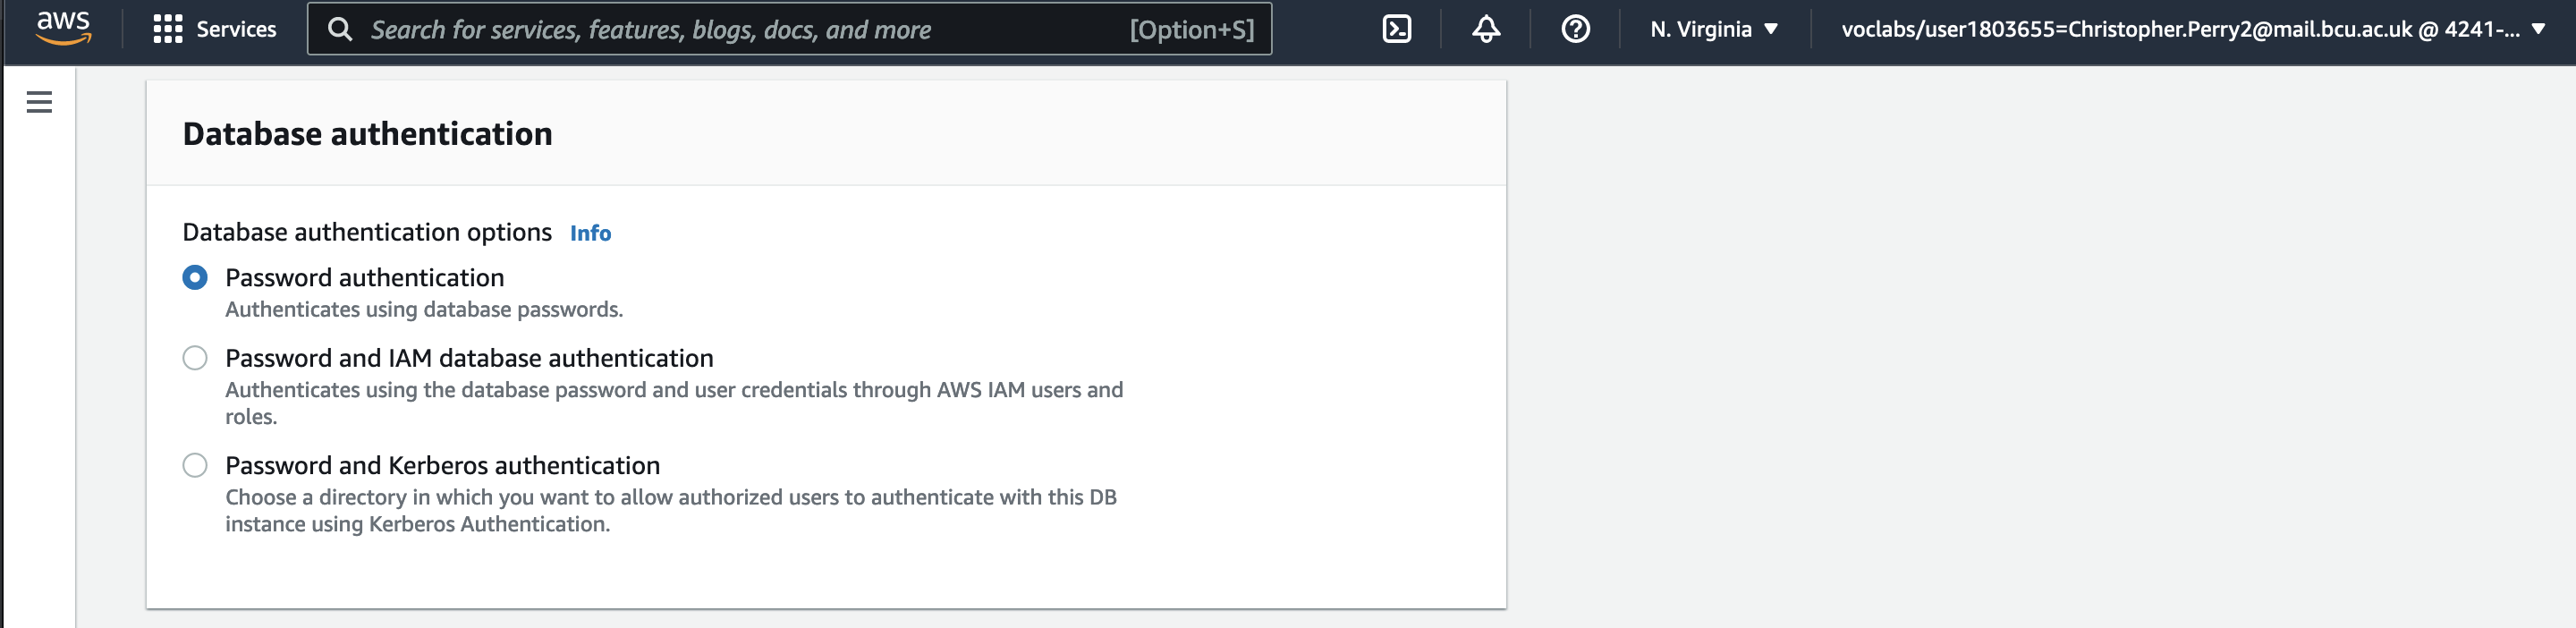
\includegraphics[width=\textwidth]{resources/rds/rds-authentication.png}
    \caption{Selection of RDS Authentication Option.}
    \label{fig:rds-auth}
\end{figure}

Password authentication was used for the RDS instance as we did not have permission from the root user to create IAM
roles within this lab environment.
In the future, it would be recommended to select one of the other options to improve security, however this was not
possible for the project.

\begin{figure}[!htbp]
    \centering
    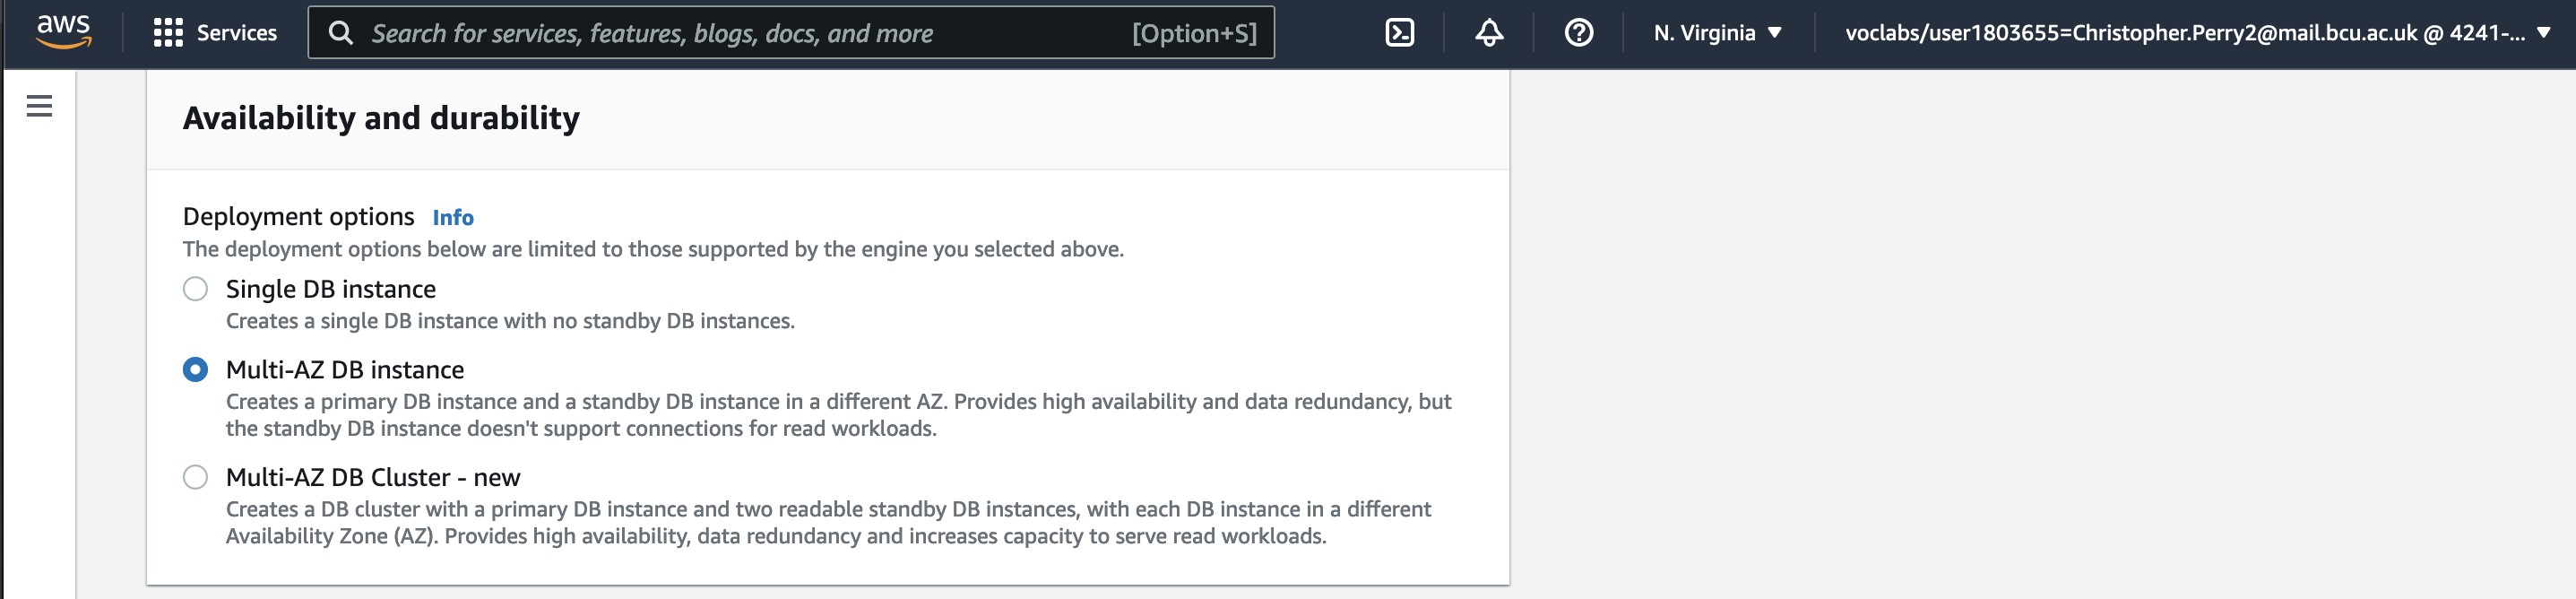
\includegraphics[width=\textwidth]{resources/rds/rds-availability-durability}
    \caption{Selection RDS Multiple Availability Zone.}
    \label{fig:rds-avail}
\end{figure}

Multiple availability zones were selected to ensure that the database was highly available.

\begin{figure}[!htbp]
    \centering
    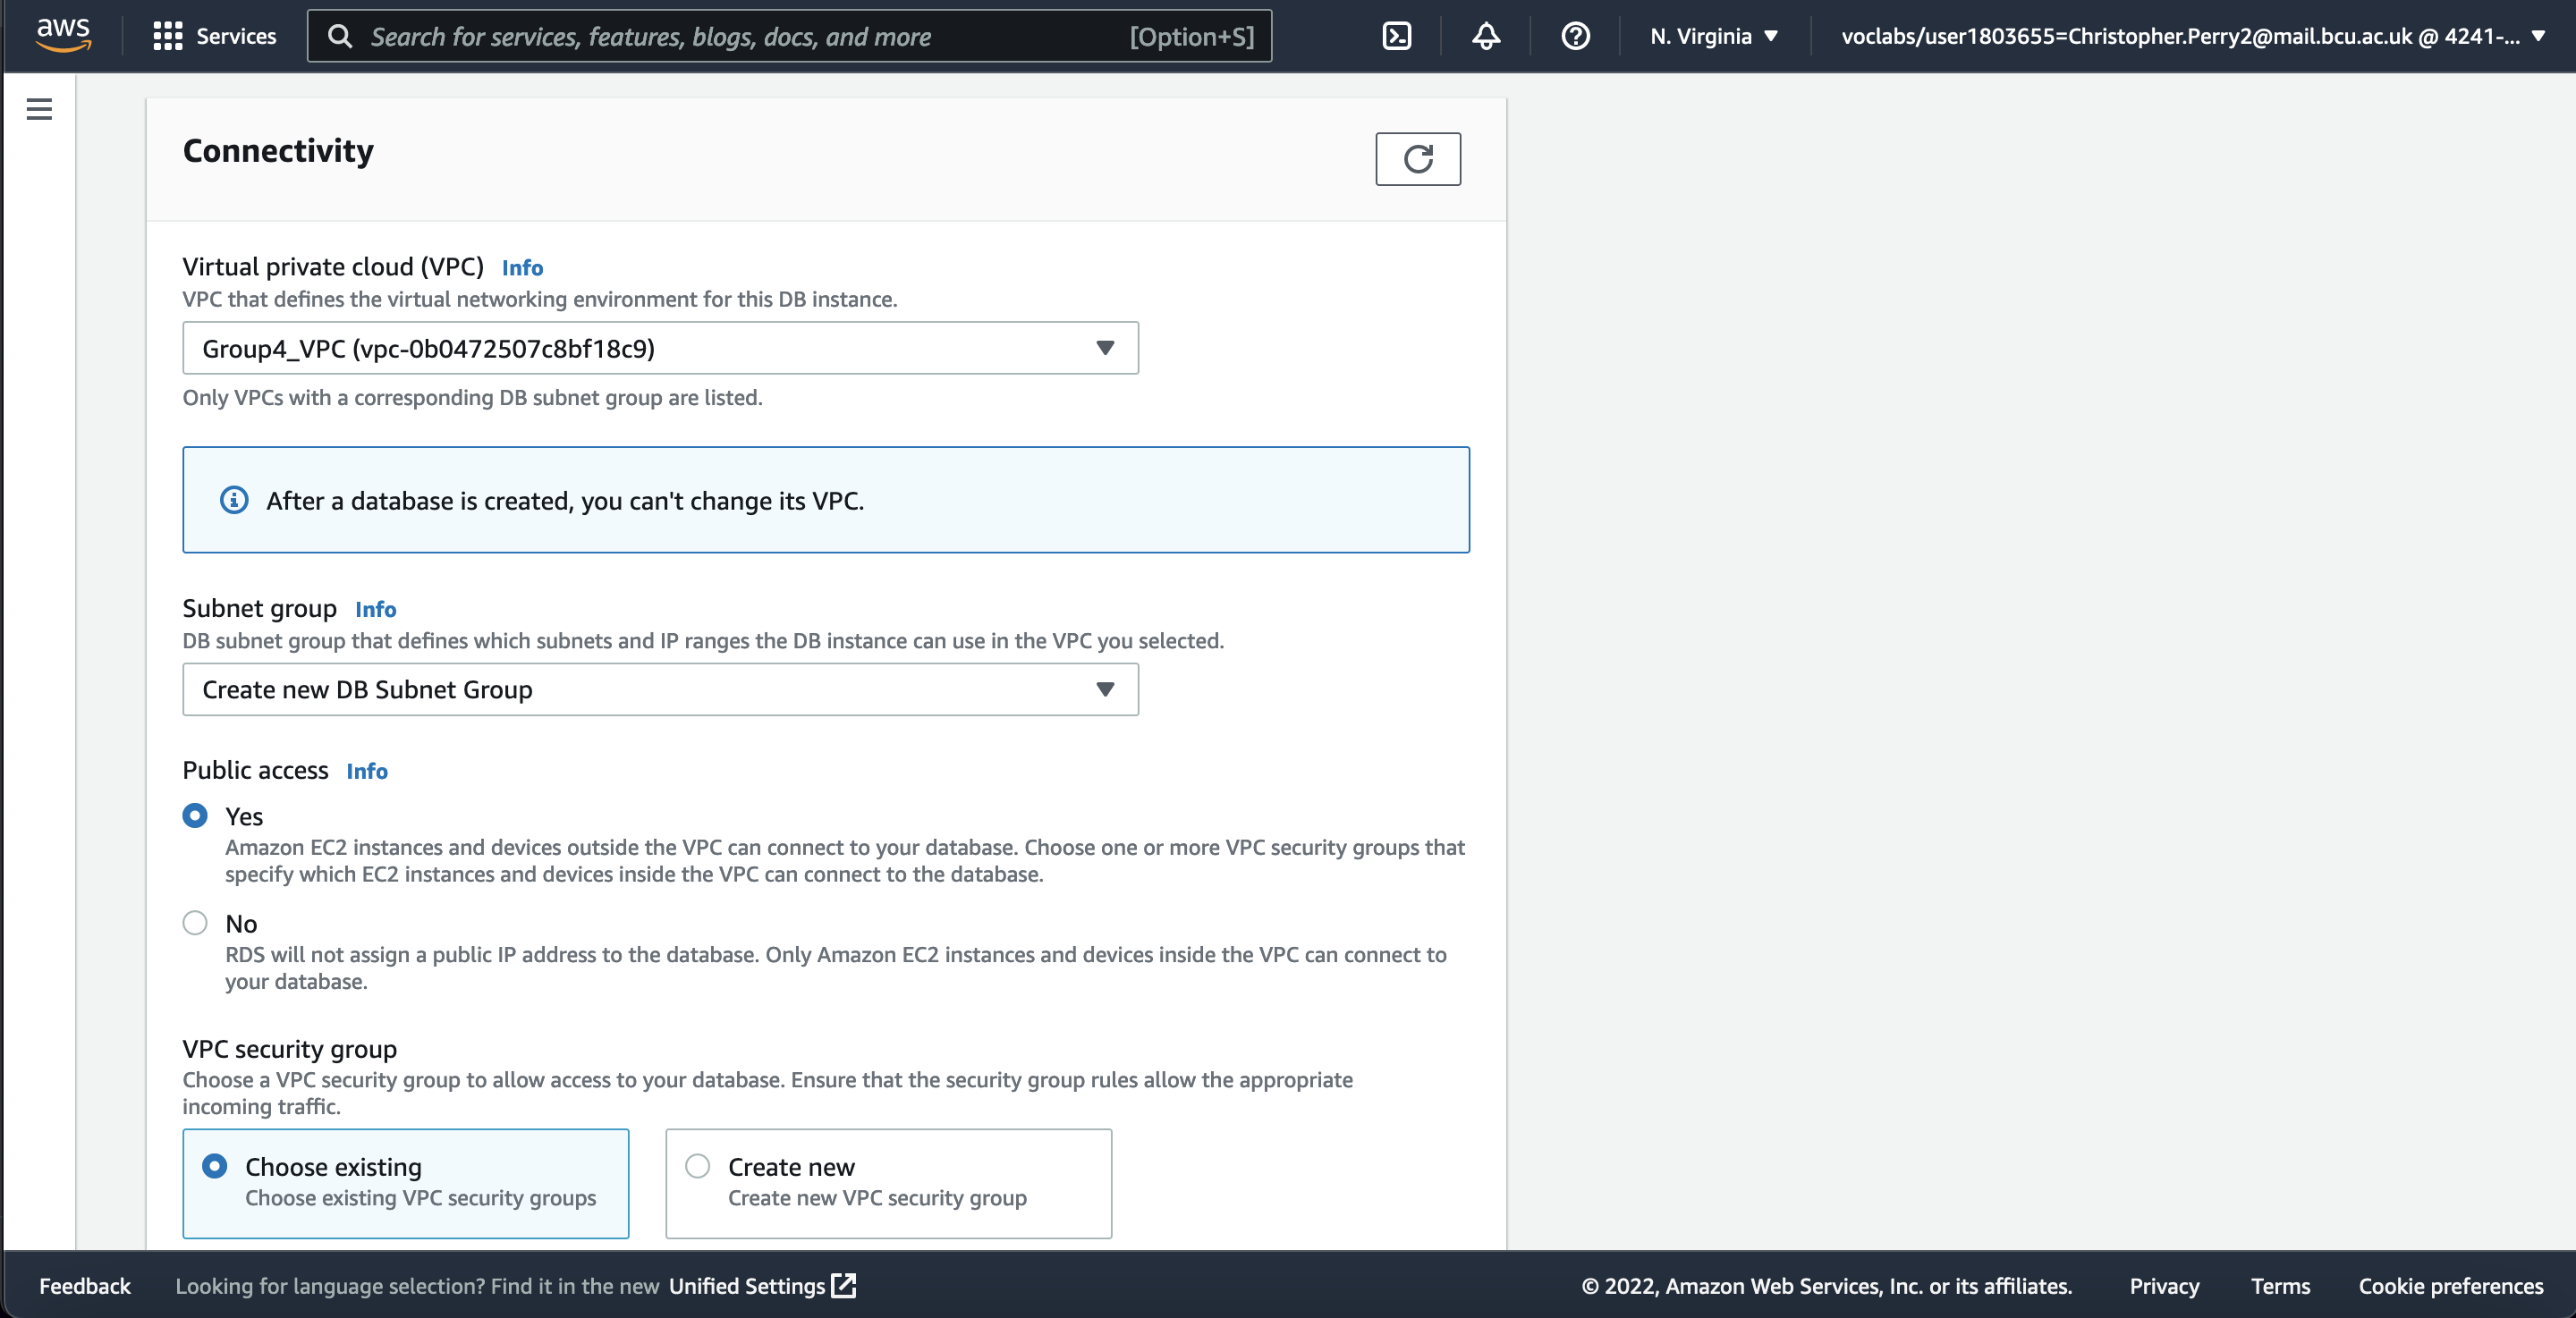
\includegraphics[width=\textwidth]{resources/rds/rds-connectivity-1}
    \caption{Selection of VPC and Subnet Groups.}
    \label{fig:rds-connecting}
\end{figure}

Public access was turned off to further increase our application's security.

\begin{figure}[!htbp]
    \centering
    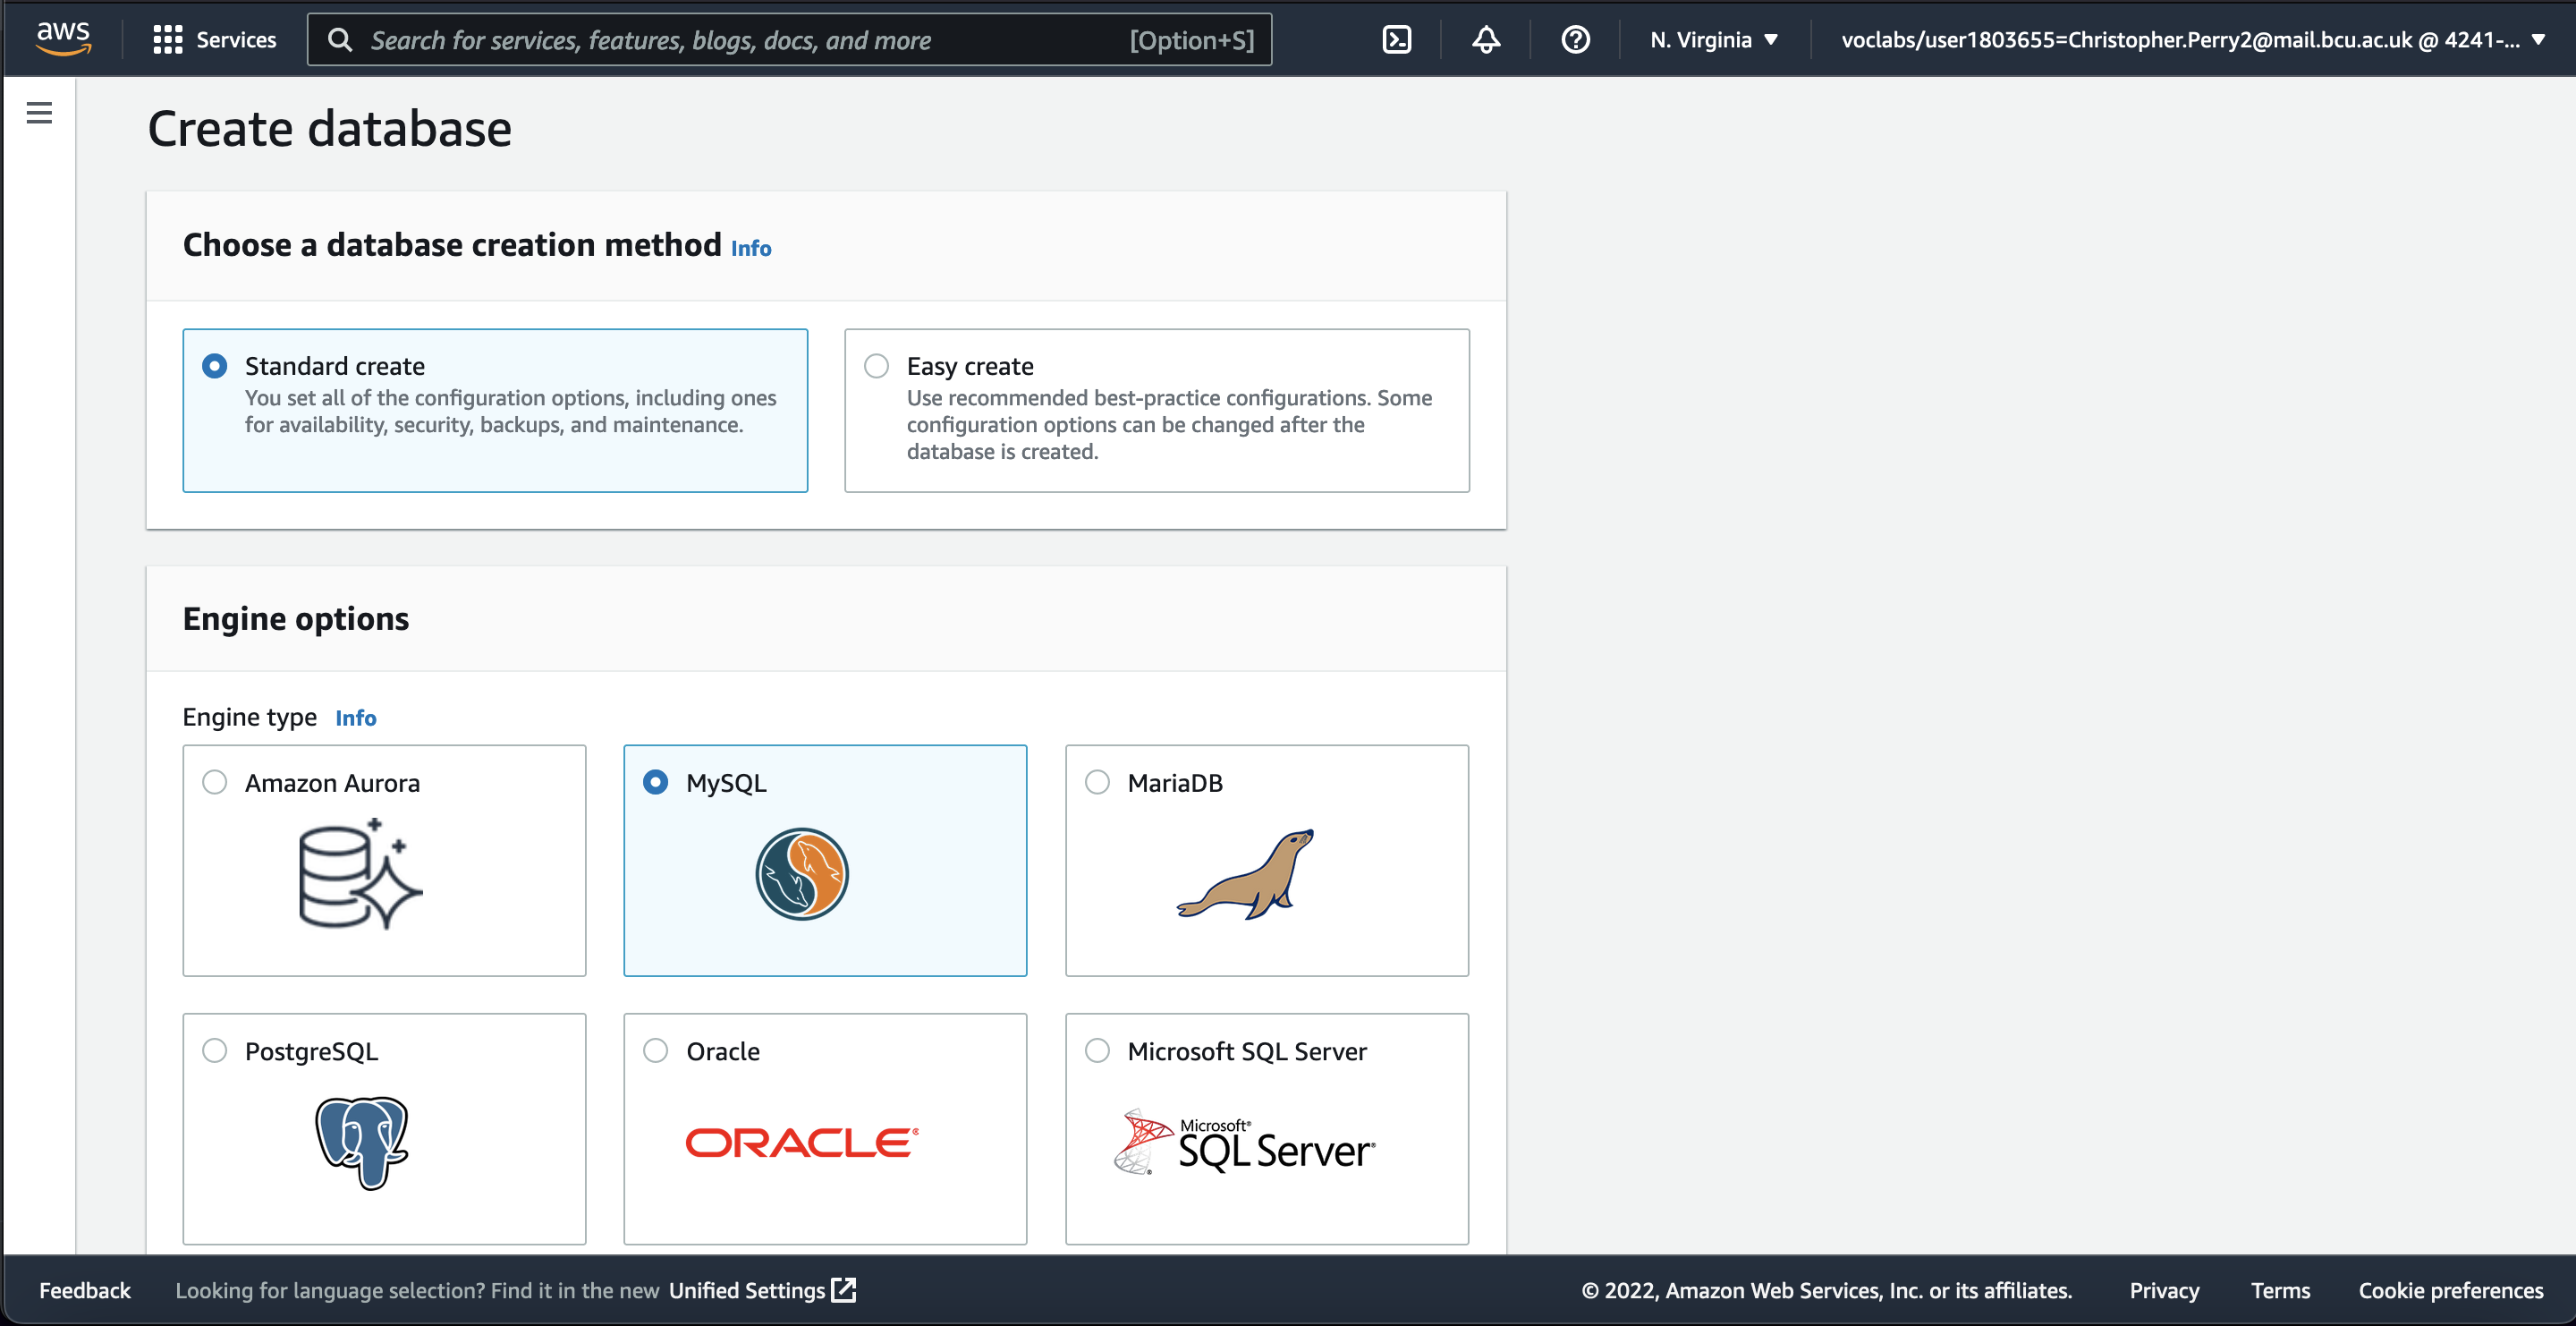
\includegraphics[width=\textwidth]{resources/rds/rds-create-engine}
    \caption{Selection of Database Engine.}
    \label{fig:rds-engine}
\end{figure}

\begin{figure}[!htbp]
    \centering
    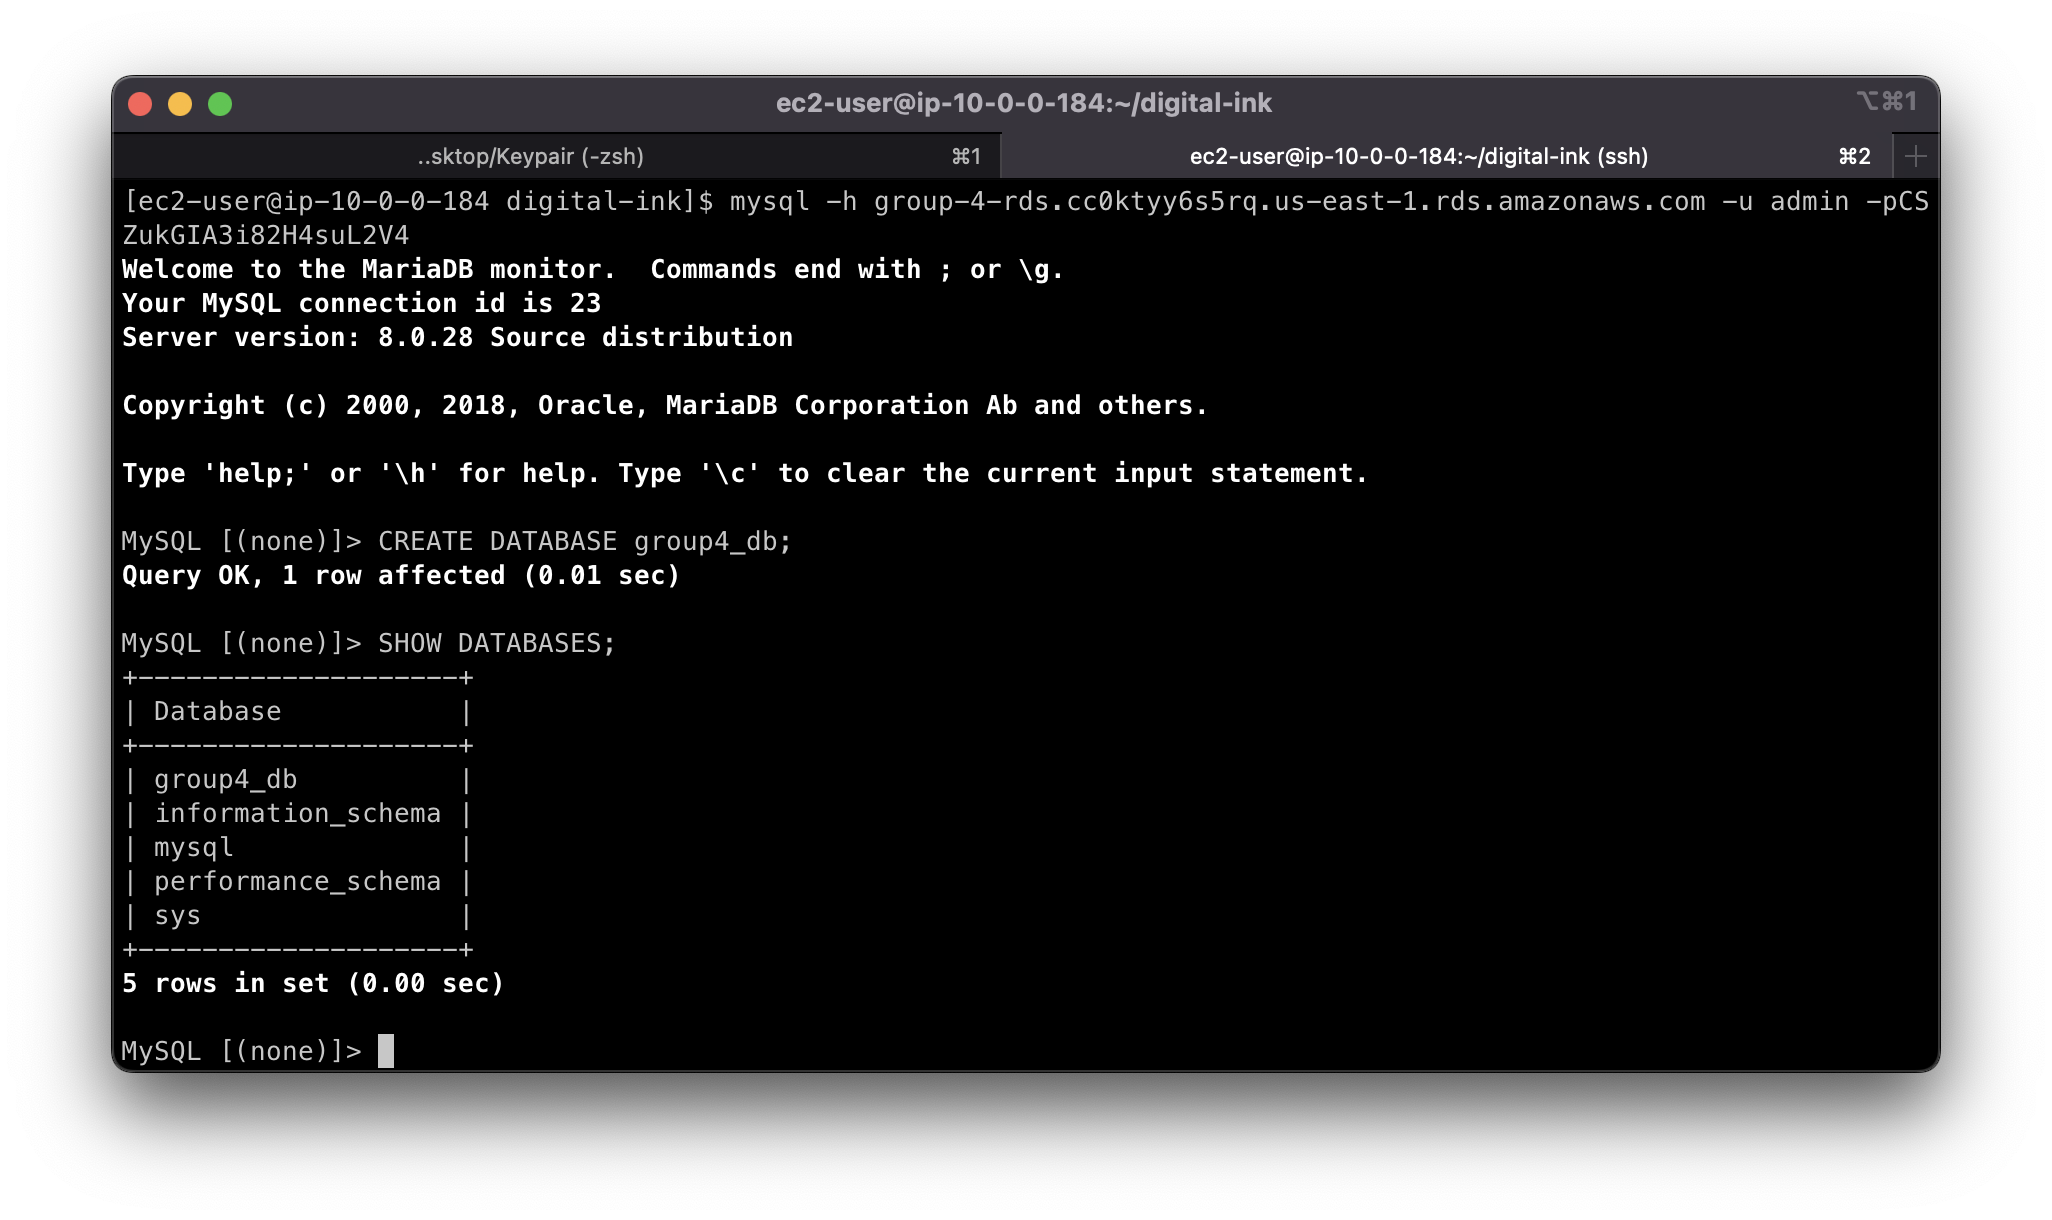
\includegraphics[width=\textwidth]{resources/rds/rds-database-creation}
    \caption{Selection of CloudWatch metric for EC2 instance.}
    \label{fig:rds-db-create}
\end{figure}

\begin{figure}[!htbp]
    \centering
    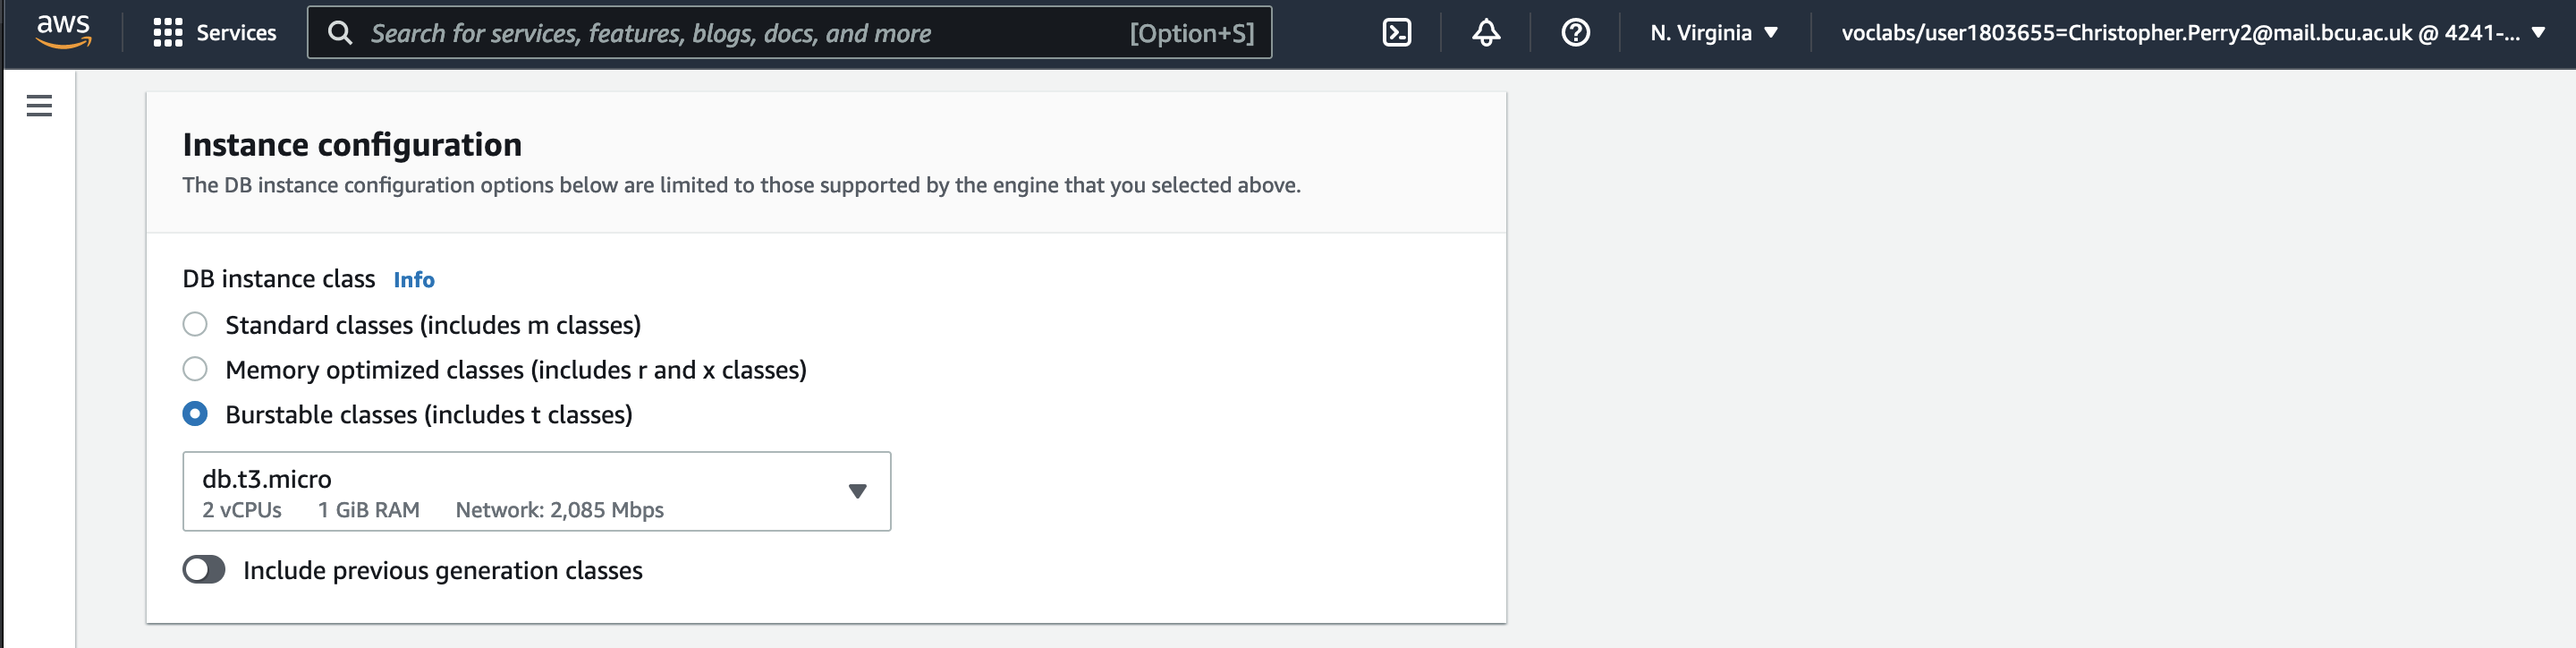
\includegraphics[width=\textwidth]{resources/rds/rds-instance-config}
    \caption{Selection of RDS Instance Size.}
    \label{fig:rds-instance-conf}
\end{figure}

A micro-sized instance was selected as we must save on AWS billing credit.

\begin{figure}[!htbp]
    \centering
    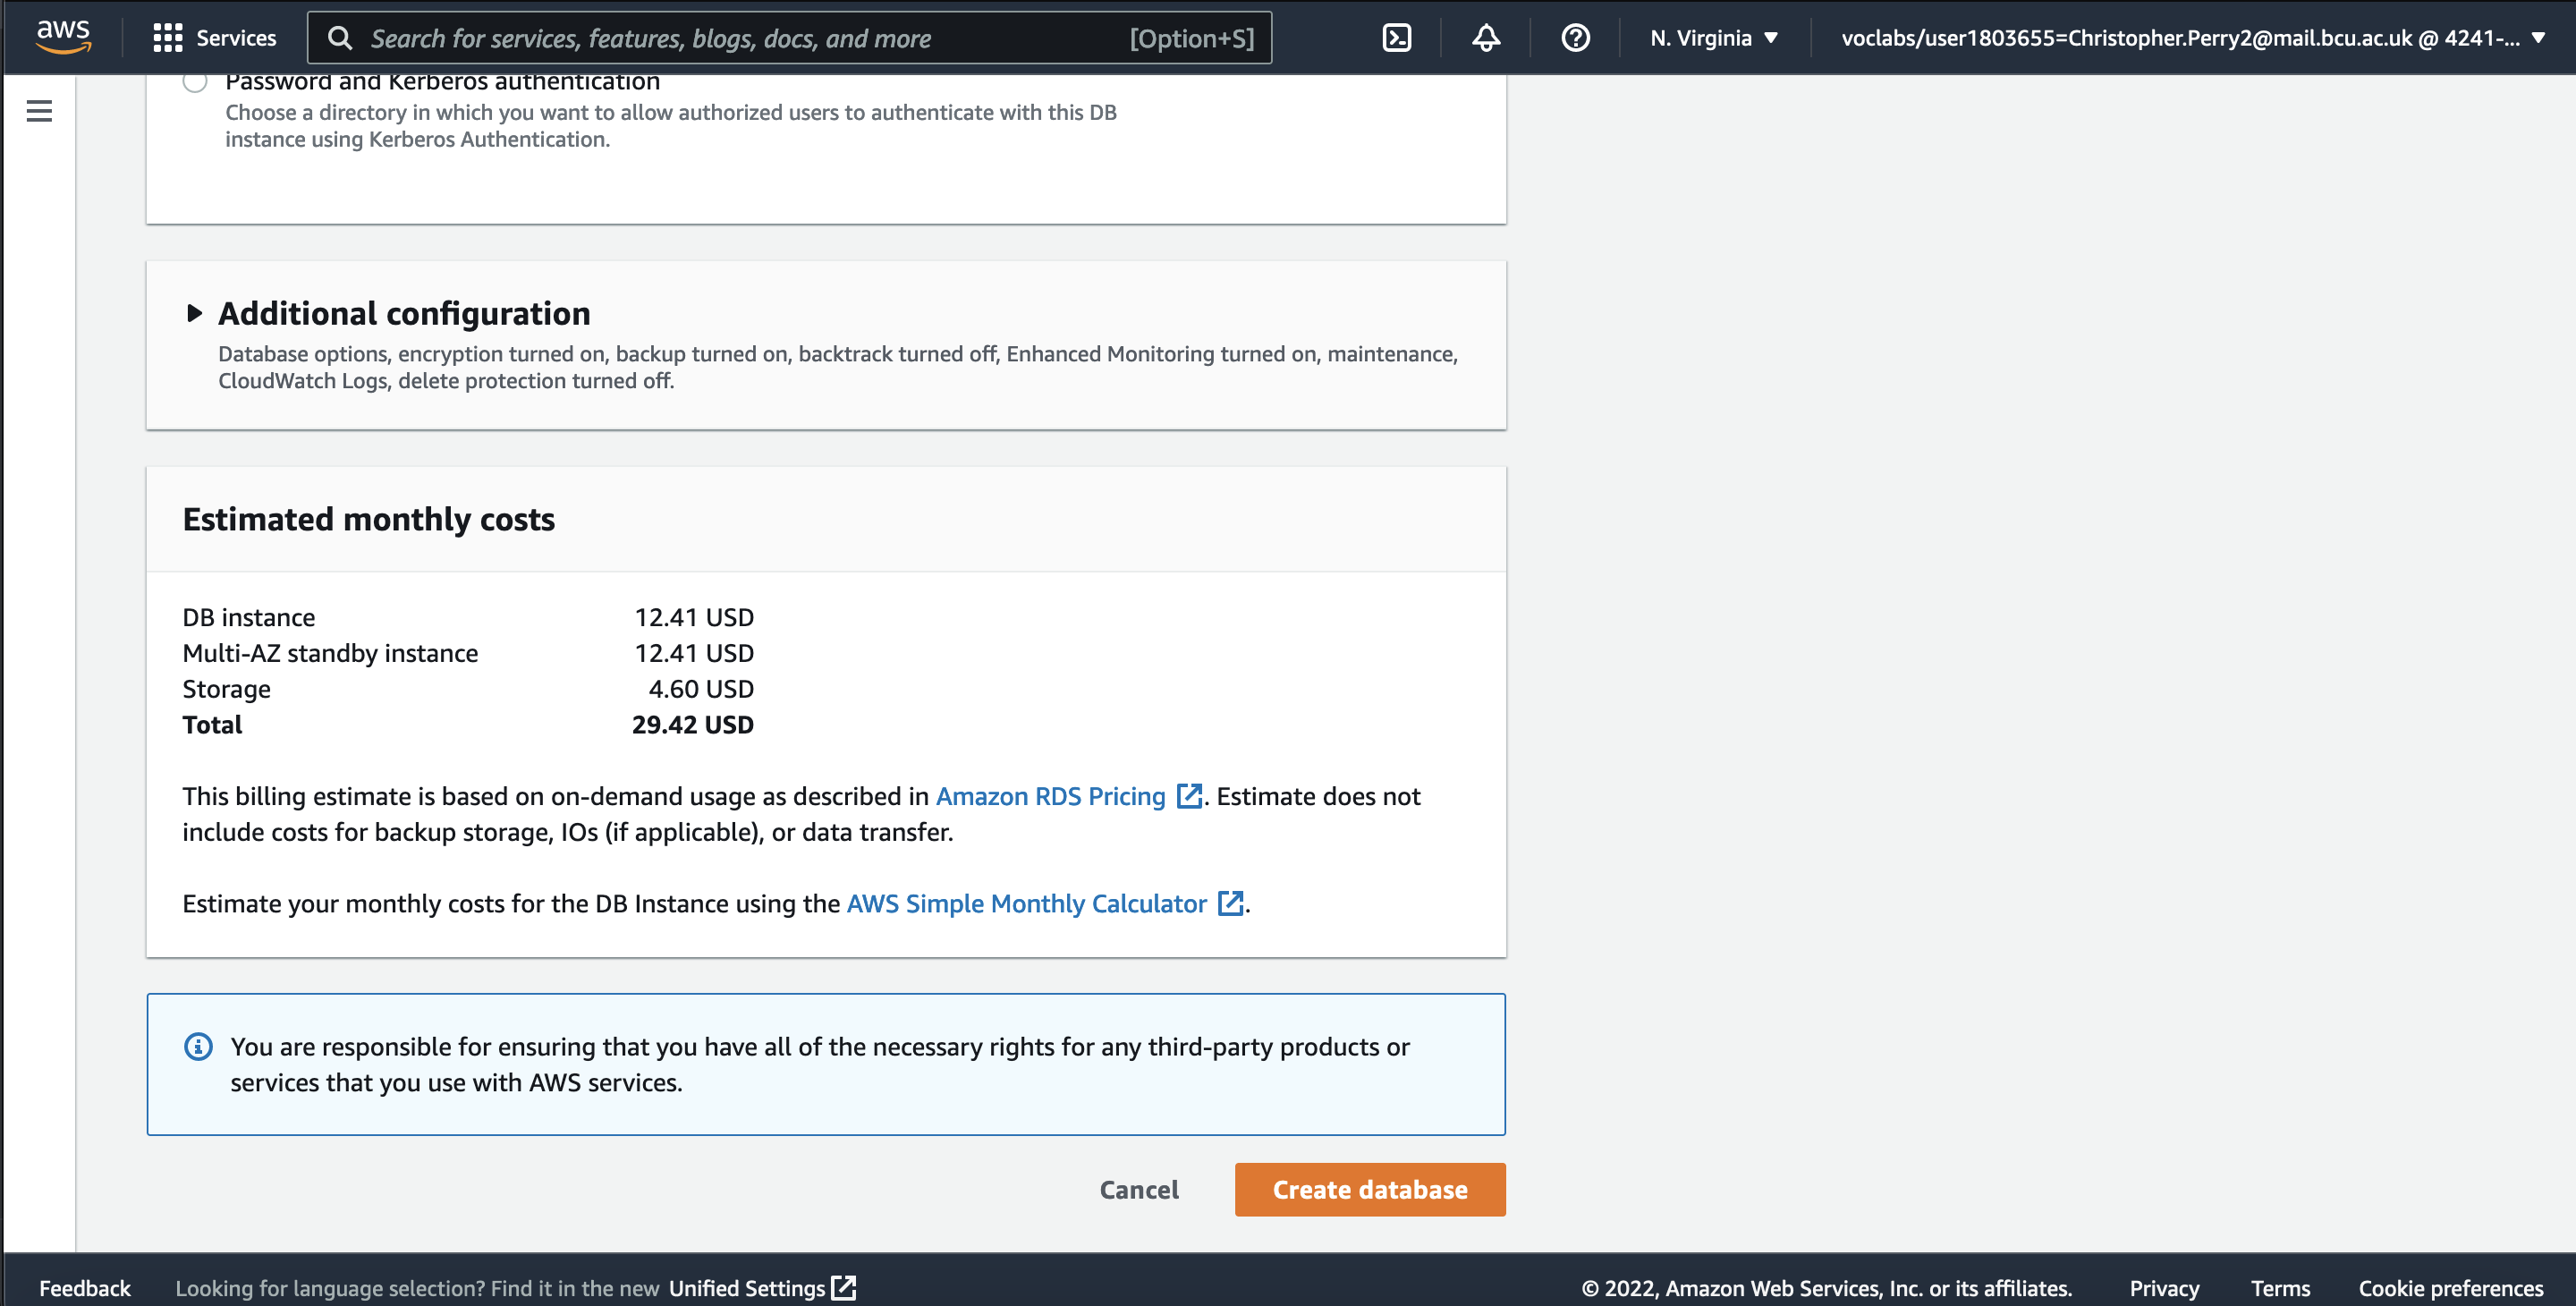
\includegraphics[width=\textwidth]{resources/rds/rds-monthly-costs}
    \caption{Estimated Monthly RDS Cost.}
    \label{fig:rds-costs}
\end{figure}

This is the estimated cost of the RDS instance for a month.

\begin{figure}[!htbp]
    \centering
    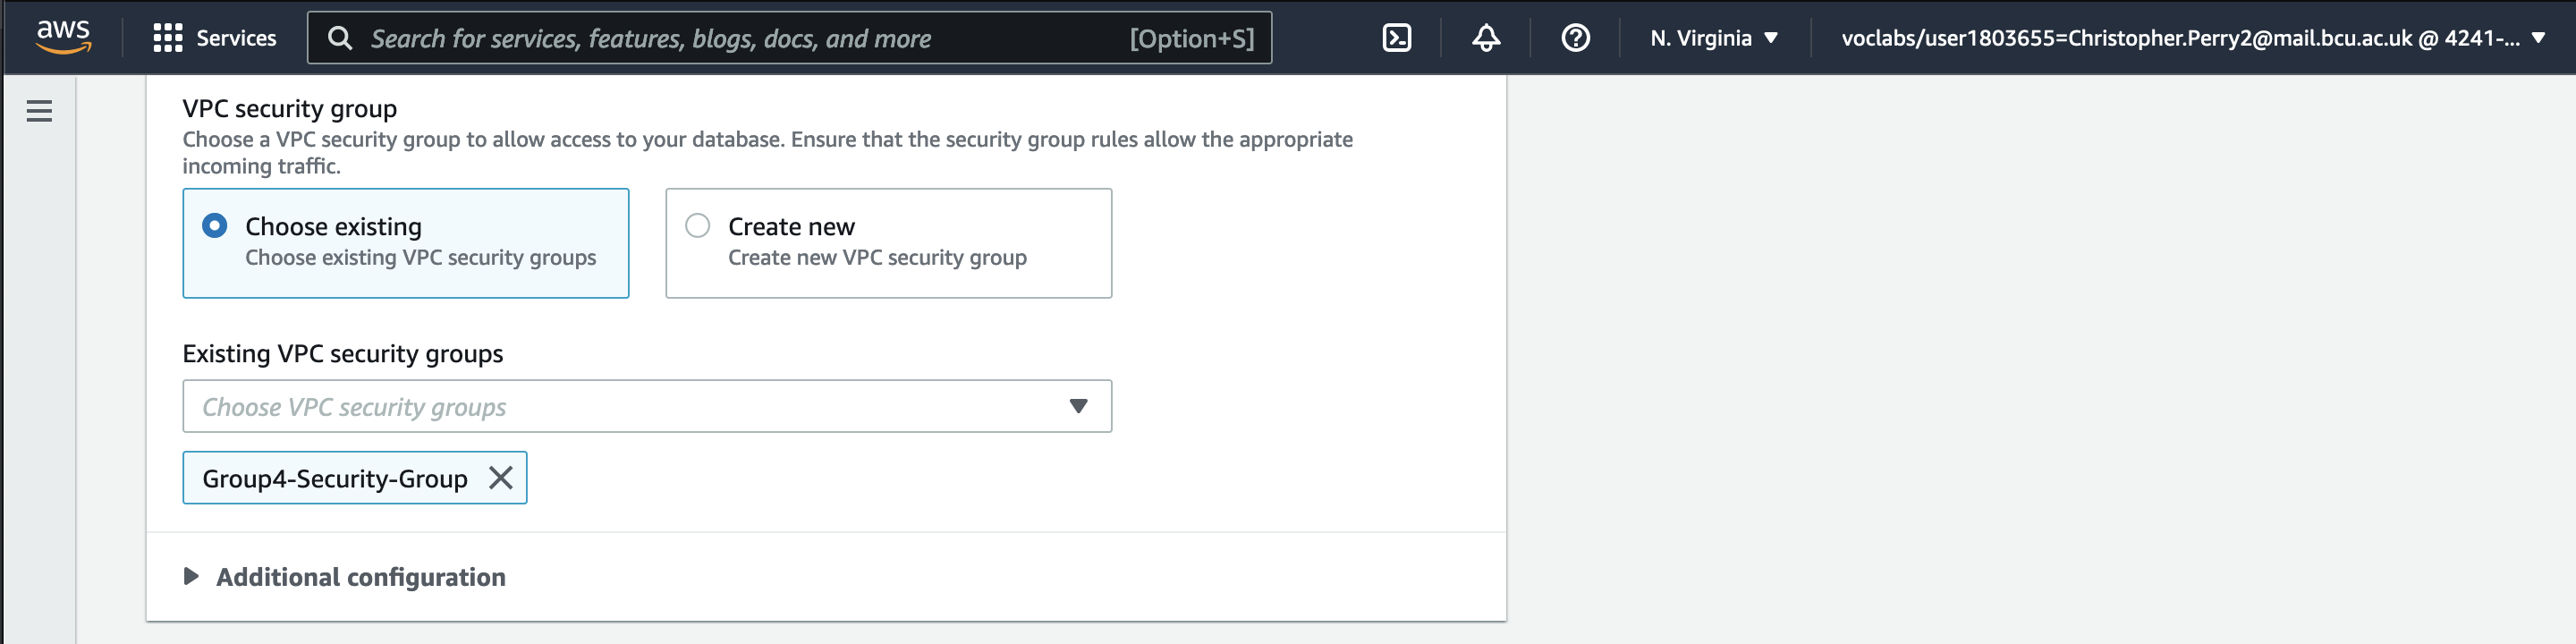
\includegraphics[width=\textwidth]{resources/rds/rds-security-group}
    \caption{Selection RDS Security Group.}
    \label{fig:rds-security}
\end{figure}

\begin{figure}[!htbp]
    \centering
    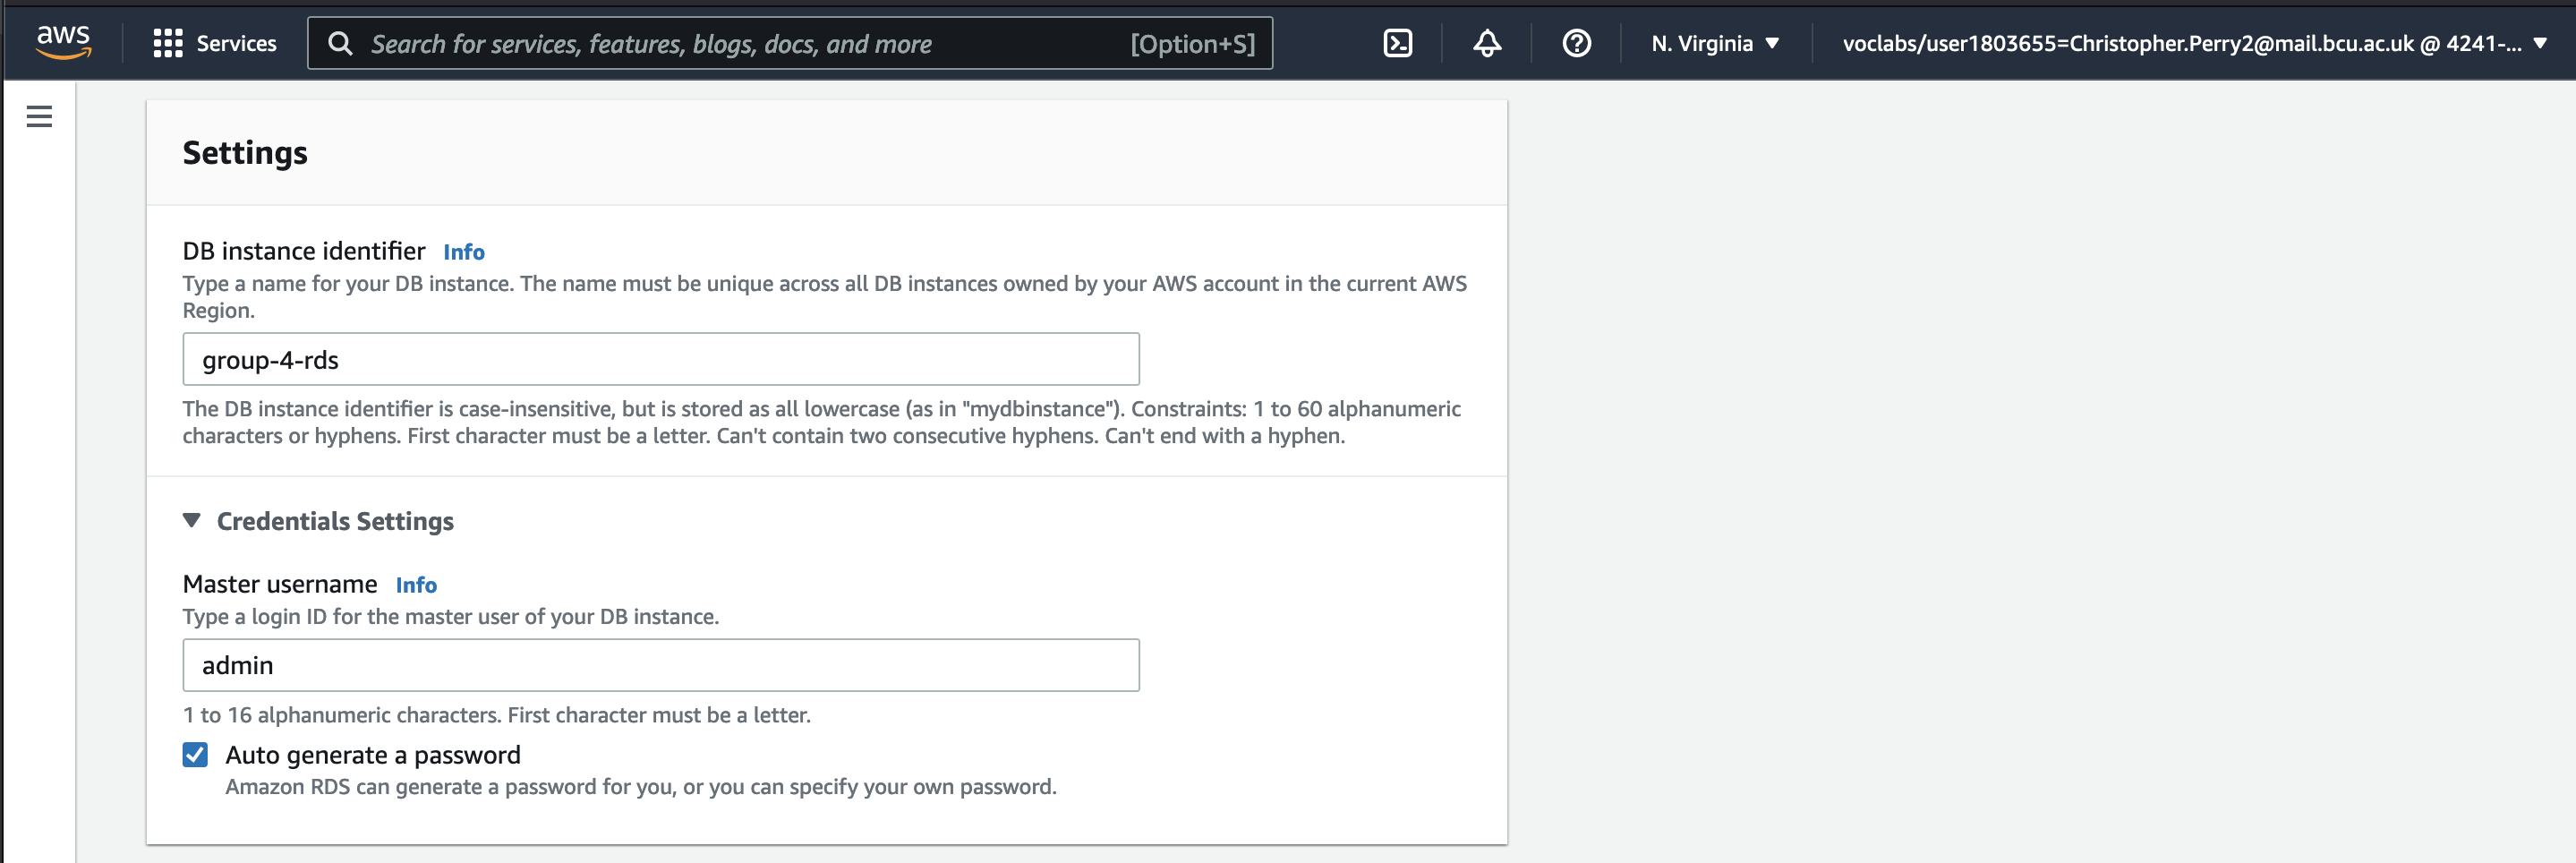
\includegraphics[width=\textwidth]{resources/rds/rds-settings}
    \caption{Credentials for RDS Authentication.}
    \label{fig:rds-settings}
\end{figure}

We selected an automatically generated password to ensure that it was created with current best security practices.

\begin{figure}[!htbp]
    \centering
    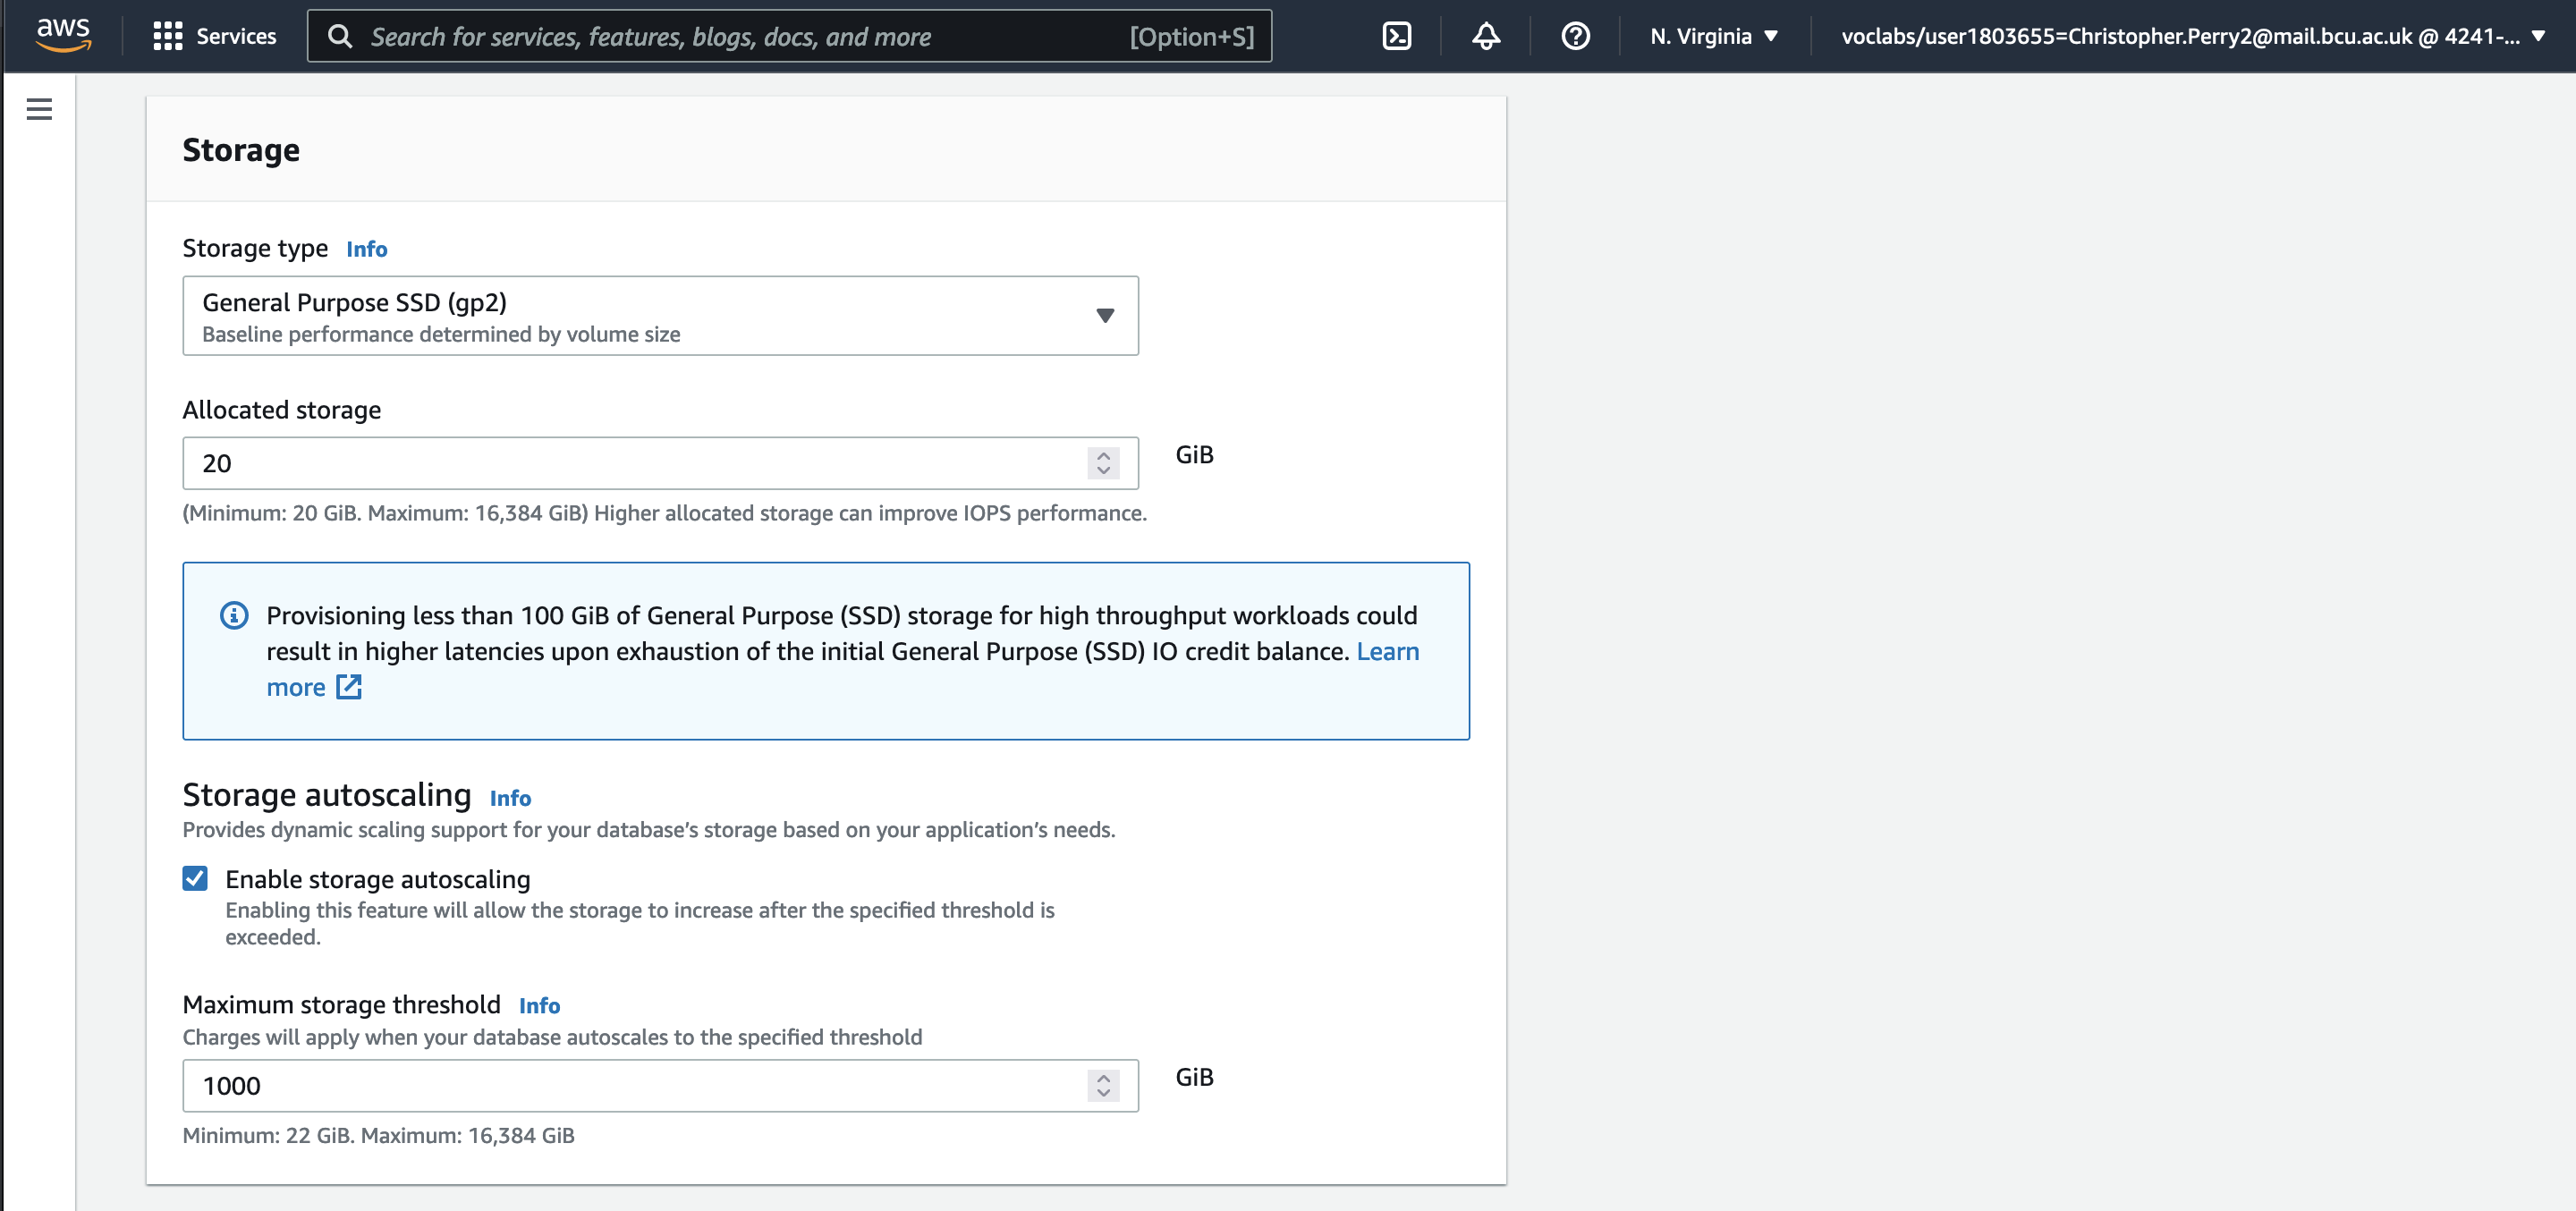
\includegraphics[width=\textwidth]{resources/rds/rds-storage}
    \caption{Selection of Storage Parameters.}
    \label{fig:rds-storage}
\end{figure}

A selection of how much storage the RDS instance is able to access should be made.
We decided that, due to billing constraints, we should go as small as possible but with size to automatically grow if
the application was presented with more users.

\begin{figure}[!htbp]
    \centering
    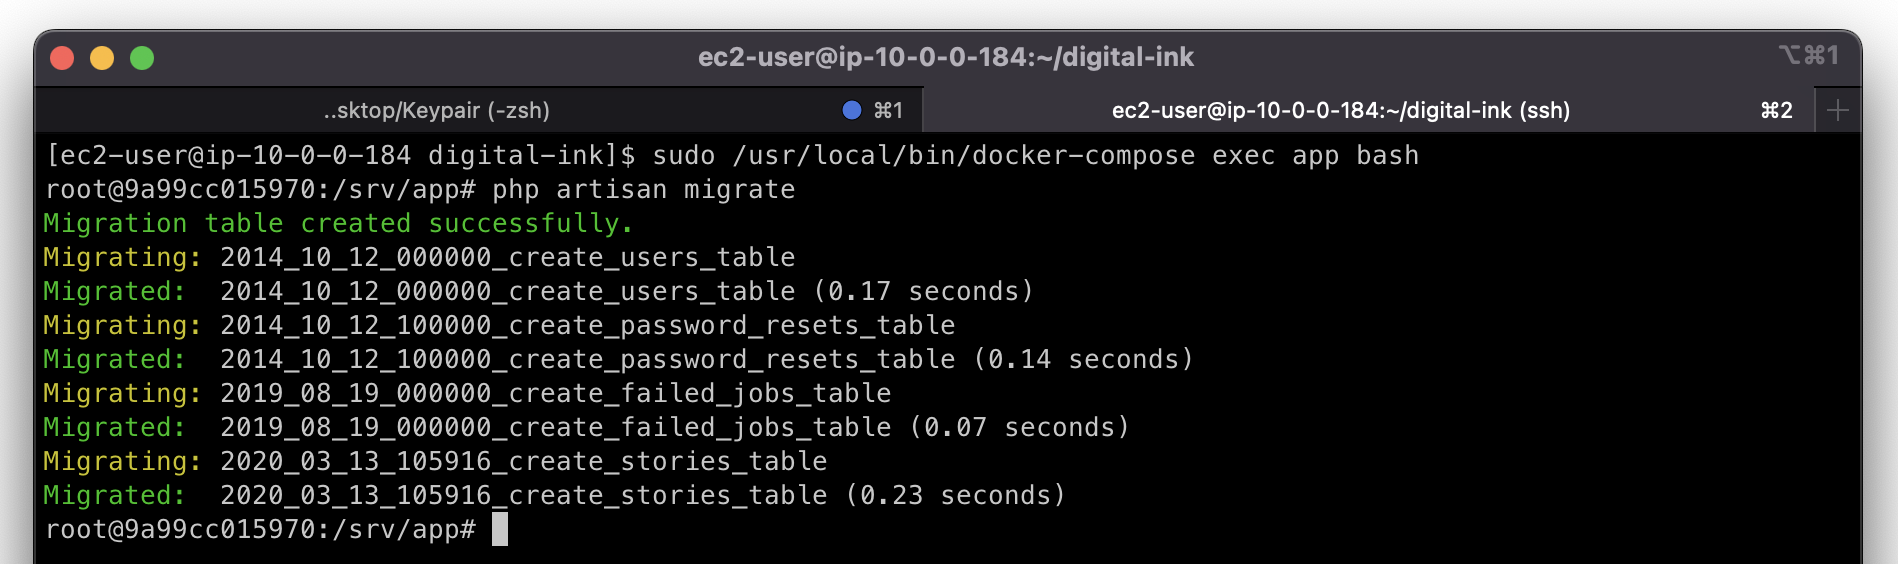
\includegraphics[width=\textwidth]{resources/rds/rds-tables-creation}
    \caption{Creation of RDS Tables.}
    \label{fig:rds-tables}
\end{figure}


\begin{figure}[!htbp]
\centering
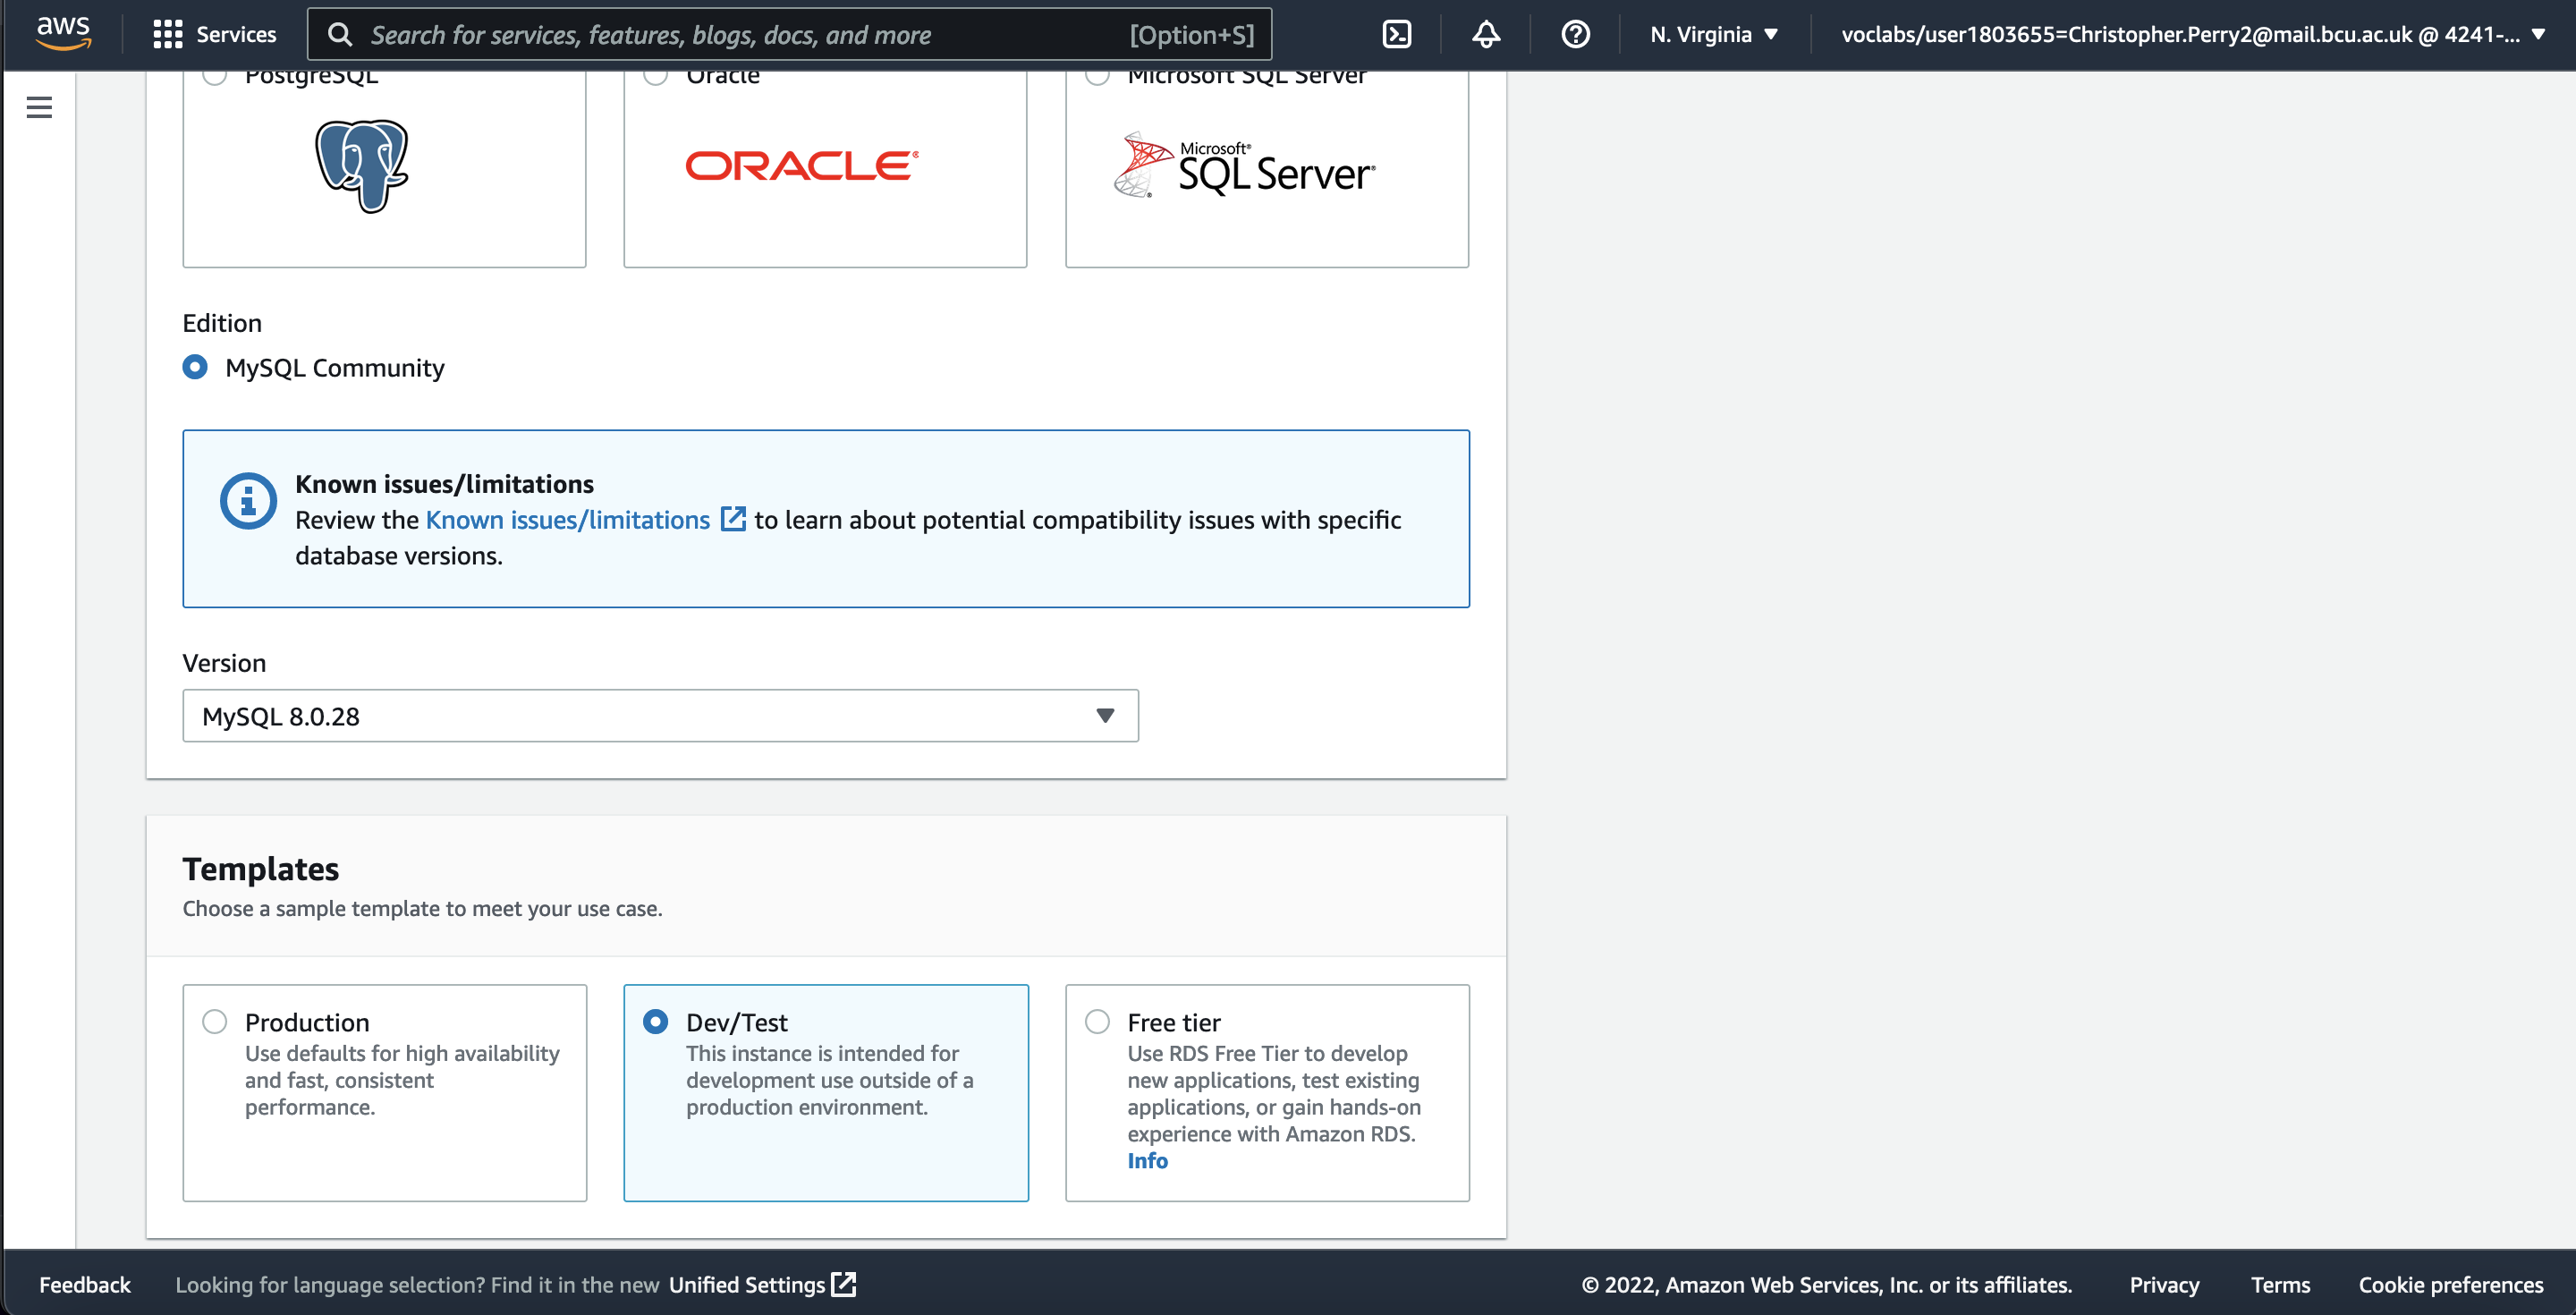
\includegraphics[width=\textwidth]{resources/rds/rds-templates}
\caption{Selection of CloudWatch metric for EC2 instance.}
\label{fig:rds-templates}
\end{figure}


MySQL was selected as it was the same database engine that the web application was originally using within Docker.

Then, MySQL was installed on the EC2 instance in order to sign in to the new database and create tables.

\begin{figure}[!htbp]
\centering
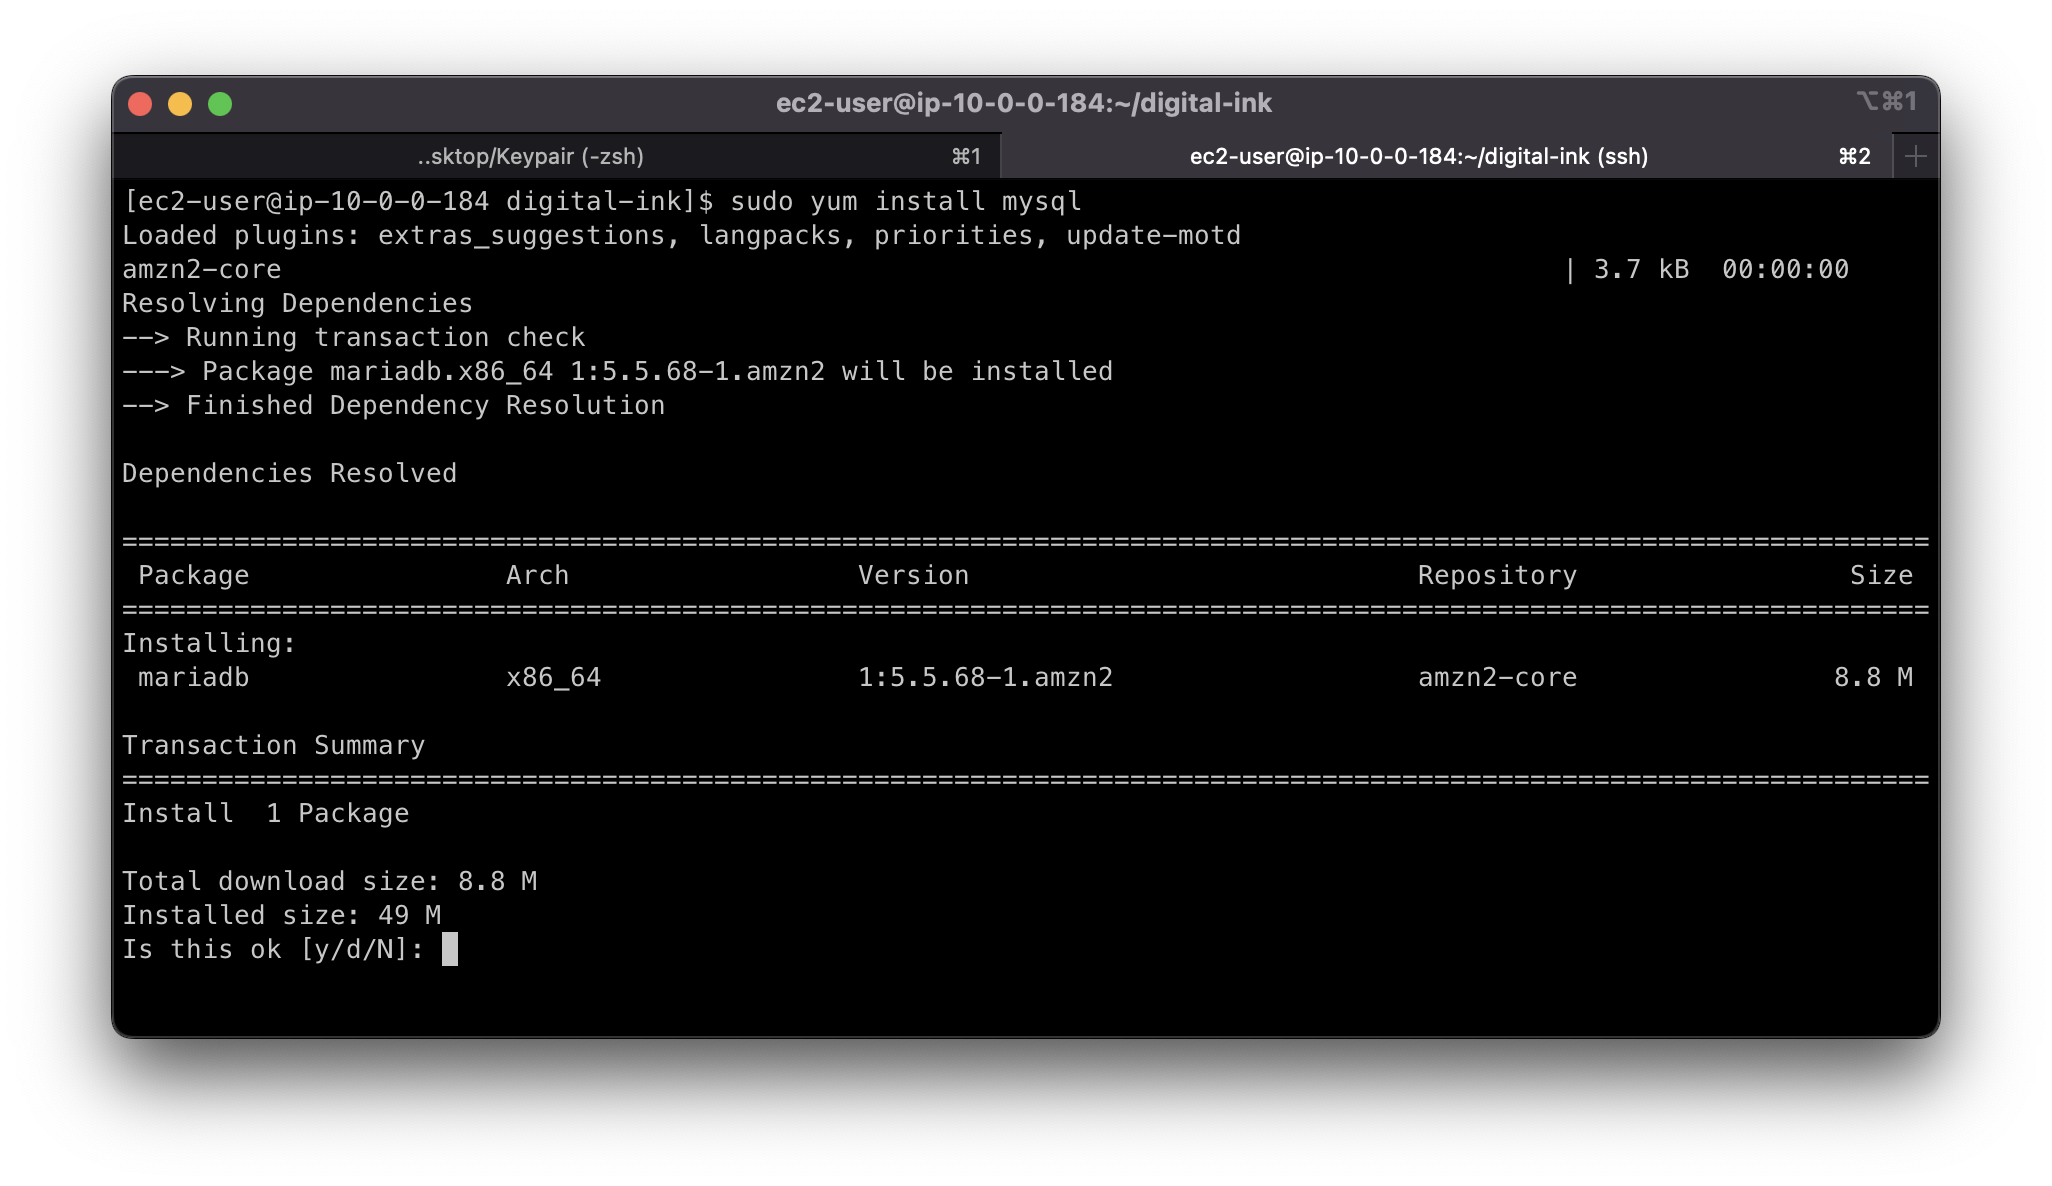
\includegraphics[width=\textwidth]{resources/rds/rds-mysql-install}
\caption{Installation of MySQL on EC2 Instance.}
\label{fig:rds-msql-install}
\end{figure}

\begin{figure}[!htbp]
\centering
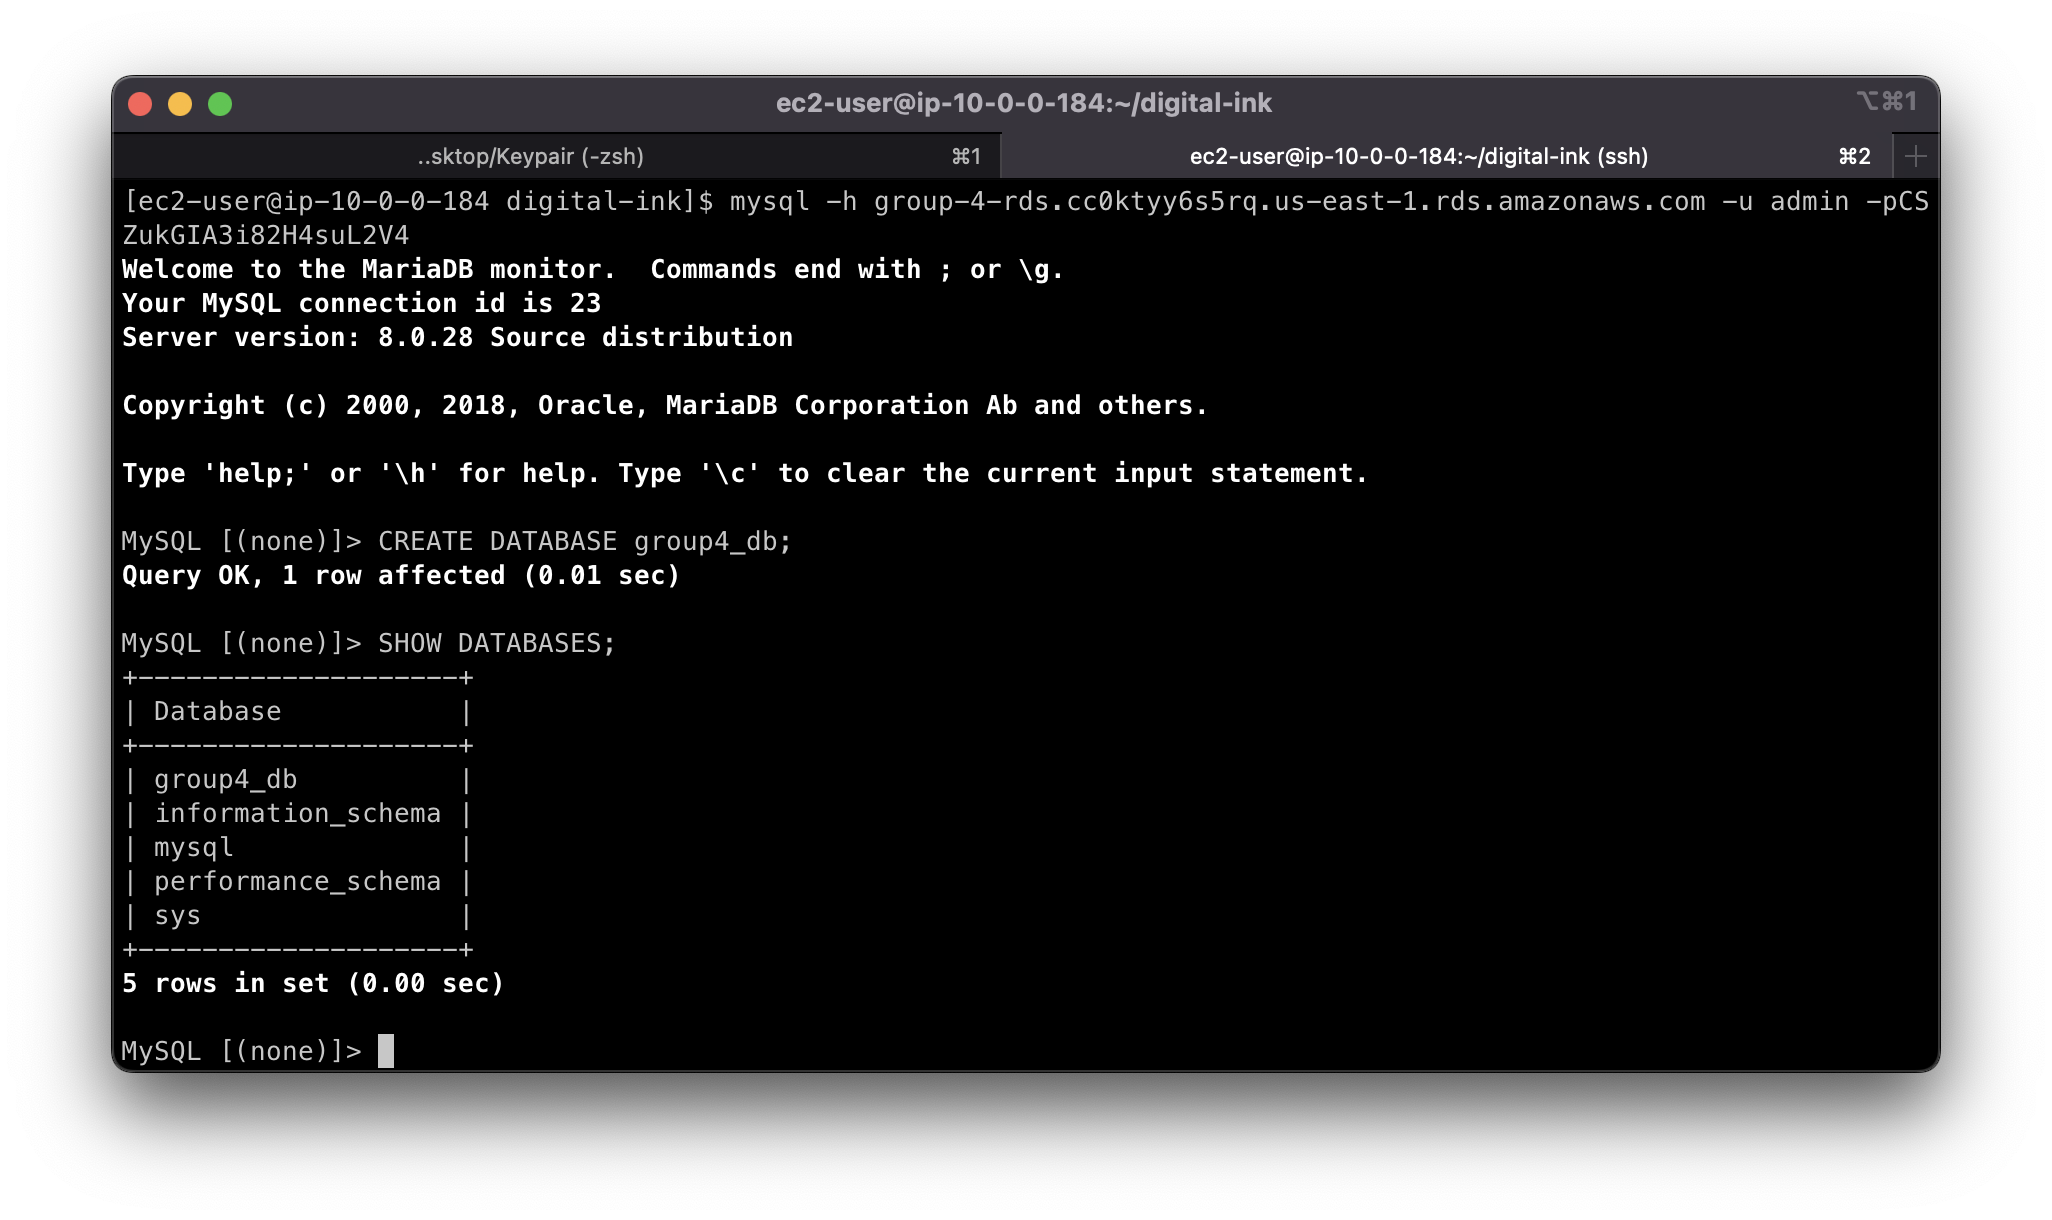
\includegraphics[width=\textwidth]{resources/rds/rds-database-creation}
\caption{Creation of database table.}
\label{fig:rds-db-create-2}
\end{figure}

\begin{figure}[!htbp]
    \centering
    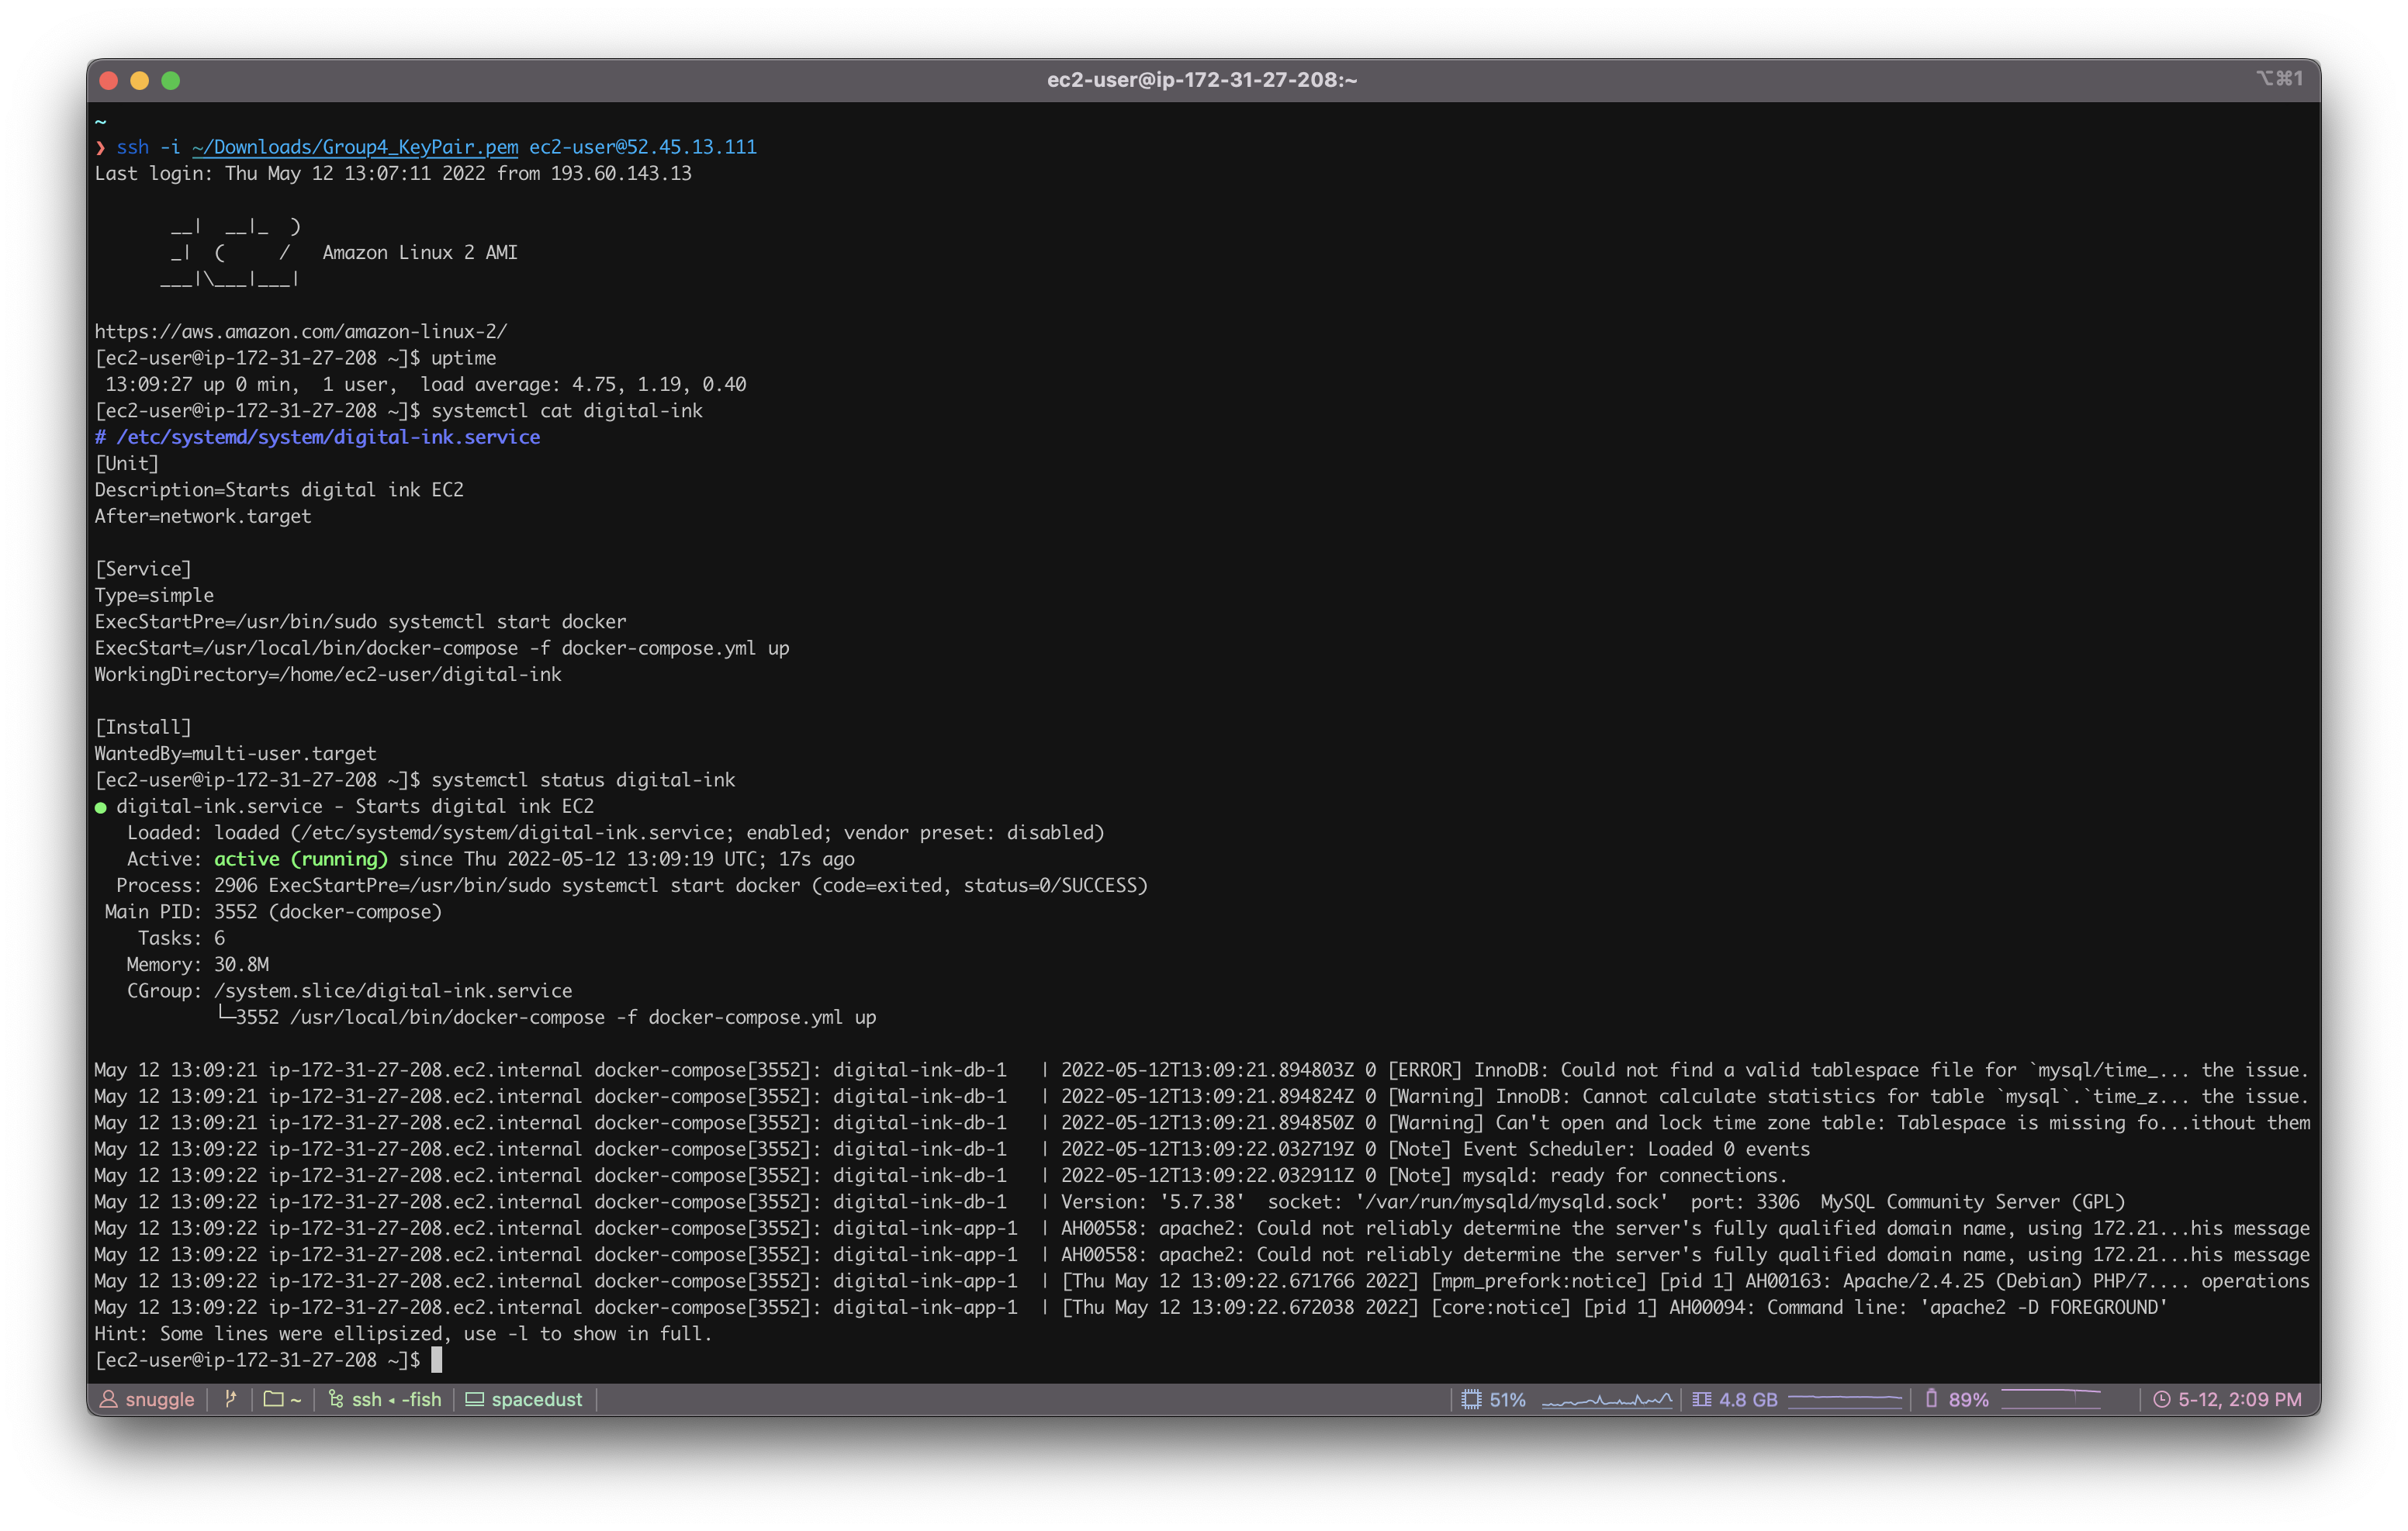
\includegraphics[width=50mm]{resources/rds/envupdate}
    \caption{Changing Database Endpoint from Docker to AWS RDS.}
    \label{fig:rds-env-update}
\end{figure}

\begin{figure}[!htbp]
    \centering
    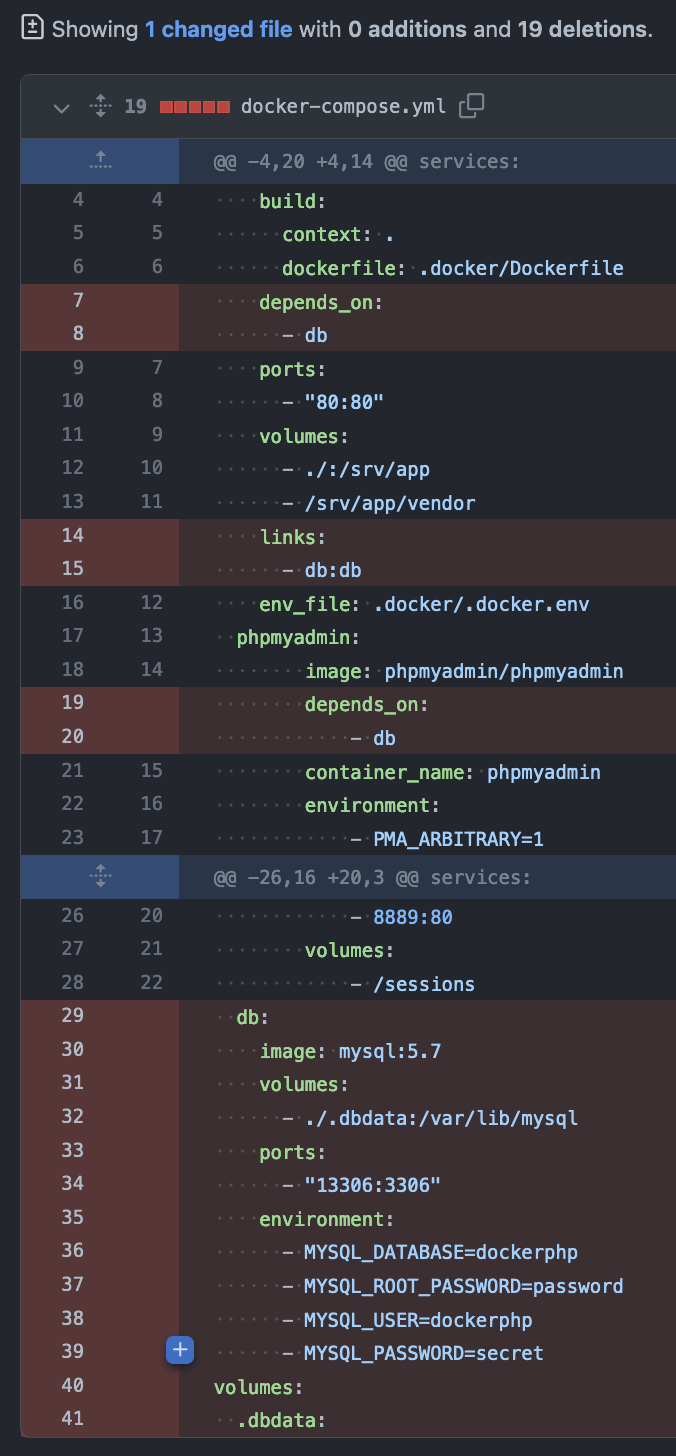
\includegraphics[width=50mm]{resources/rds/docker}
    \caption{Removal of Database from Docker File.}
    \label{fig:rds-rm-docker-compose}
\end{figure}

After the database was set up, tested and working, we were able to remove the old MySQL docker container from the
docker-compose file.